% Options for packages loaded elsewhere
\PassOptionsToPackage{unicode}{hyperref}
\PassOptionsToPackage{hyphens}{url}
%
\documentclass[
  a4paper,
  oneside,
  openany]{book}
\usepackage{amsmath,amssymb}
\usepackage{lmodern}
\usepackage{iftex}
\ifPDFTeX
  \usepackage[T1]{fontenc}
  \usepackage[utf8]{inputenc}
  \usepackage{textcomp} % provide euro and other symbols
\else % if luatex or xetex
  \usepackage{unicode-math}
  \defaultfontfeatures{Scale=MatchLowercase}
  \defaultfontfeatures[\rmfamily]{Ligatures=TeX,Scale=1}
\fi
% Use upquote if available, for straight quotes in verbatim environments
\IfFileExists{upquote.sty}{\usepackage{upquote}}{}
\IfFileExists{microtype.sty}{% use microtype if available
  \usepackage[]{microtype}
  \UseMicrotypeSet[protrusion]{basicmath} % disable protrusion for tt fonts
}{}
\makeatletter
\@ifundefined{KOMAClassName}{% if non-KOMA class
  \IfFileExists{parskip.sty}{%
    \usepackage{parskip}
  }{% else
    \setlength{\parindent}{0pt}
    \setlength{\parskip}{6pt plus 2pt minus 1pt}}
}{% if KOMA class
  \KOMAoptions{parskip=half}}
\makeatother
\usepackage{xcolor}
\IfFileExists{xurl.sty}{\usepackage{xurl}}{} % add URL line breaks if available
\IfFileExists{bookmark.sty}{\usepackage{bookmark}}{\usepackage{hyperref}}
\hypersetup{
  pdftitle={Análisis de Series de Tiempo},
  pdfauthor={Sofía Villers Gómez; David Alberto Mateos Montes de Oca; Carlos Fernando Vásquez Guerra},
  hidelinks,
  pdfcreator={LaTeX via pandoc}}
\urlstyle{same} % disable monospaced font for URLs
\usepackage[top=1in, left=1in, right=1in, bottom=1in]{geometry}
\usepackage{color}
\usepackage{fancyvrb}
\newcommand{\VerbBar}{|}
\newcommand{\VERB}{\Verb[commandchars=\\\{\}]}
\DefineVerbatimEnvironment{Highlighting}{Verbatim}{commandchars=\\\{\}}
% Add ',fontsize=\small' for more characters per line
\usepackage{framed}
\definecolor{shadecolor}{RGB}{248,248,248}
\newenvironment{Shaded}{\begin{snugshade}}{\end{snugshade}}
\newcommand{\AlertTok}[1]{\textcolor[rgb]{0.94,0.16,0.16}{#1}}
\newcommand{\AnnotationTok}[1]{\textcolor[rgb]{0.56,0.35,0.01}{\textbf{\textit{#1}}}}
\newcommand{\AttributeTok}[1]{\textcolor[rgb]{0.77,0.63,0.00}{#1}}
\newcommand{\BaseNTok}[1]{\textcolor[rgb]{0.00,0.00,0.81}{#1}}
\newcommand{\BuiltInTok}[1]{#1}
\newcommand{\CharTok}[1]{\textcolor[rgb]{0.31,0.60,0.02}{#1}}
\newcommand{\CommentTok}[1]{\textcolor[rgb]{0.56,0.35,0.01}{\textit{#1}}}
\newcommand{\CommentVarTok}[1]{\textcolor[rgb]{0.56,0.35,0.01}{\textbf{\textit{#1}}}}
\newcommand{\ConstantTok}[1]{\textcolor[rgb]{0.00,0.00,0.00}{#1}}
\newcommand{\ControlFlowTok}[1]{\textcolor[rgb]{0.13,0.29,0.53}{\textbf{#1}}}
\newcommand{\DataTypeTok}[1]{\textcolor[rgb]{0.13,0.29,0.53}{#1}}
\newcommand{\DecValTok}[1]{\textcolor[rgb]{0.00,0.00,0.81}{#1}}
\newcommand{\DocumentationTok}[1]{\textcolor[rgb]{0.56,0.35,0.01}{\textbf{\textit{#1}}}}
\newcommand{\ErrorTok}[1]{\textcolor[rgb]{0.64,0.00,0.00}{\textbf{#1}}}
\newcommand{\ExtensionTok}[1]{#1}
\newcommand{\FloatTok}[1]{\textcolor[rgb]{0.00,0.00,0.81}{#1}}
\newcommand{\FunctionTok}[1]{\textcolor[rgb]{0.00,0.00,0.00}{#1}}
\newcommand{\ImportTok}[1]{#1}
\newcommand{\InformationTok}[1]{\textcolor[rgb]{0.56,0.35,0.01}{\textbf{\textit{#1}}}}
\newcommand{\KeywordTok}[1]{\textcolor[rgb]{0.13,0.29,0.53}{\textbf{#1}}}
\newcommand{\NormalTok}[1]{#1}
\newcommand{\OperatorTok}[1]{\textcolor[rgb]{0.81,0.36,0.00}{\textbf{#1}}}
\newcommand{\OtherTok}[1]{\textcolor[rgb]{0.56,0.35,0.01}{#1}}
\newcommand{\PreprocessorTok}[1]{\textcolor[rgb]{0.56,0.35,0.01}{\textit{#1}}}
\newcommand{\RegionMarkerTok}[1]{#1}
\newcommand{\SpecialCharTok}[1]{\textcolor[rgb]{0.00,0.00,0.00}{#1}}
\newcommand{\SpecialStringTok}[1]{\textcolor[rgb]{0.31,0.60,0.02}{#1}}
\newcommand{\StringTok}[1]{\textcolor[rgb]{0.31,0.60,0.02}{#1}}
\newcommand{\VariableTok}[1]{\textcolor[rgb]{0.00,0.00,0.00}{#1}}
\newcommand{\VerbatimStringTok}[1]{\textcolor[rgb]{0.31,0.60,0.02}{#1}}
\newcommand{\WarningTok}[1]{\textcolor[rgb]{0.56,0.35,0.01}{\textbf{\textit{#1}}}}
\usepackage{longtable,booktabs,array}
\usepackage{calc} % for calculating minipage widths
% Correct order of tables after \paragraph or \subparagraph
\usepackage{etoolbox}
\makeatletter
\patchcmd\longtable{\par}{\if@noskipsec\mbox{}\fi\par}{}{}
\makeatother
% Allow footnotes in longtable head/foot
\IfFileExists{footnotehyper.sty}{\usepackage{footnotehyper}}{\usepackage{footnote}}
\makesavenoteenv{longtable}
\usepackage{graphicx}
\makeatletter
\def\maxwidth{\ifdim\Gin@nat@width>\linewidth\linewidth\else\Gin@nat@width\fi}
\def\maxheight{\ifdim\Gin@nat@height>\textheight\textheight\else\Gin@nat@height\fi}
\makeatother
% Scale images if necessary, so that they will not overflow the page
% margins by default, and it is still possible to overwrite the defaults
% using explicit options in \includegraphics[width, height, ...]{}
\setkeys{Gin}{width=\maxwidth,height=\maxheight,keepaspectratio}
% Set default figure placement to htbp
\makeatletter
\def\fps@figure{htbp}
\makeatother
\setlength{\emergencystretch}{3em} % prevent overfull lines
\providecommand{\tightlist}{%
  \setlength{\itemsep}{0pt}\setlength{\parskip}{0pt}}
\setcounter{secnumdepth}{5}
\usepackage[utf8]{inputenc}% Usa codificación 8-bit que tiene 256 glyphs
\usepackage[T1]{fontenc}
%Más información de babel : http://www.texnia.com/spanishopt.html
%es-tabla: Traduce table como tabla en lugar de como cuadro.
%es-nodecimaldot: No añade punto tras los números de sección, subsección
\usepackage[spanish,es-nodecimaldot,es-tabla]{babel} 
\usepackage{graphicx} %Manipulación de imágenes : https://es.overleaf.com/learn/latex/Inserting_Images
\usepackage{tikz} % Requerido para dibujar formas personalizadas
\usepackage{float} %Gráficas
\usepackage{fancyhdr} %Para un mejor manejo de encabezados
\usepackage{calc} %Para hacer cálculos matemáticos en Latex
\usepackage{amsmath,amssymb,amsfonts} %Para tener mejores opciones en estructuras matemáticas.
\usepackage{amsthm} %Ambientes matemáticos : http://www.ctex.org/documents/packages/math/amsthdoc.pdf
%Vamos a colocar todo el formato que yihui colocó en su bookdown:https://github.com/rstudio/bookdown/blob/master/inst/examples/latex/preamble.tex
\usepackage{mathrsfs}
\usepackage{booktabs}
\usepackage{longtable}
\renewcommand{\textfraction}{0.05}
\renewcommand{\topfraction}{0.8}
\renewcommand{\bottomfraction}{0.8}
\renewcommand{\floatpagefraction}{0.75}
\usepackage{listings}
\lstset{
  breaklines=true
}
\usepackage{booktabs}
\usepackage{longtable}
\usepackage{array}
\usepackage{multirow}
\usepackage{wrapfig}
\usepackage{float}
\usepackage{colortbl}
\usepackage{pdflscape}
\usepackage{tabu}
\usepackage{threeparttable}
\usepackage{threeparttablex}
\usepackage[normalem]{ulem}
\usepackage{makecell}
\usepackage{xcolor}
\ifLuaTeX
  \usepackage{selnolig}  % disable illegal ligatures
\fi
\usepackage[]{natbib}
\bibliographystyle{apalike}
\nocite{cryer2008time, nielsen2019practical, hyndman2018forecasting, holmes2019applied, william2006time}

\title{Análisis de Series de Tiempo}
\author{Sofía Villers Gómez \and David Alberto Mateos Montes de Oca \and Carlos Fernando Vásquez Guerra}
\date{}

\begin{document}
\maketitle

{
\setcounter{tocdepth}{3}
\tableofcontents
}
\hypertarget{prefacio}{%
\chapter*{Prefacio}\label{prefacio}}


Primera edición del bookdown \emph{Análisis de Series de Tiempo} para su uso en la materia Análisis de Supervivencia y Series de tiempo y sus relacionadas impartidas por los autores, así como para aquellos estudiantes que deseen adquirir el conocimiento pertinente de tal tópico.

\hypertarget{objetivos}{%
\subsection*{Objetivos}\label{objetivos}}


\begin{itemize}
\item
  Otorgar un material electrónico de calidad con el contenido referente al Análisis de Series de Tiempo como un esfuerzo de los autores para lograr un proceso de aprendizaje autodidacta por parte del alumno y así optimizar el tiempo, tanto de los profesores, como el de los alumnos.
\item
  Plasmar las bases teóricas de esta rama de la estadística con el uso de ejemplos y contenido visual para un mejor entendimiento de cada subtema que se trate.
\item
  Dar continuidad al material para el curso \emph{Análisis de Supervivencia y Series de Tiempo}.
\end{itemize}

\hypertarget{estructura}{%
\subsection*{Estructura}\label{estructura}}


Este libro se compone de 13 capítulos. Se recomienda que la consulta de los capítulos se realice de acuerdo al índice, ya que a medida que se avanza en índice, se asume el conocimiento de los capítulos previos.

\hypertarget{detalles-tuxe9cnicos}{%
\subsection*{Detalles técnicos}\label{detalles-tuxe9cnicos}}


Para la creación de este material se hizo uso de varios sistemas de software como LaTeX y CSS para el diseño de ciertos elementos. Todos los cálculos y gráficas fue creado con el lenguaje de programación \texttt{R} ya sea con el uso del paquete \texttt{base} o algún otro de los paquetes que se mencionan a continuación.

\begin{Shaded}
\begin{Highlighting}[]
\NormalTok{R version 4.2.1 (2022{-}06{-}23 ucrt)}
\NormalTok{Platform: x86\_64{-}w64{-}mingw32/x64 (64{-}bit)}
\NormalTok{Running under: Windows 10 x64 (build 18363)}

\NormalTok{Matrix products: default}

\NormalTok{locale:}
\NormalTok{[1] LC\_COLLATE=Spanish\_Mexico.utf8  LC\_CTYPE=Spanish\_Mexico.utf8   }
\NormalTok{[3] LC\_MONETARY=Spanish\_Mexico.utf8 LC\_NUMERIC=C                   }
\NormalTok{[5] LC\_TIME=Spanish\_Mexico.utf8    }

\NormalTok{attached base packages:}
\NormalTok{[1] stats     graphics  grDevices utils     datasets  methods   base     }

\NormalTok{other attached packages:}
\NormalTok{ [1] TSA\_1.3.1        forecast\_8.21    kableExtra\_1.3.4 knitr\_1.39      }
\NormalTok{ [5] latex2exp\_0.9.6  patchwork\_1.1.2  forcats\_0.5.1    stringr\_1.4.0   }
\NormalTok{ [9] dplyr\_1.0.9      purrr\_0.3.4      readr\_2.1.2      tidyr\_1.2.0     }
\NormalTok{[13] tibble\_3.1.7     ggplot2\_3.3.6    tidyverse\_1.3.1 }

\NormalTok{loaded via a namespace (and not attached):}
\NormalTok{ [1] tseries\_0.10{-}54   httr\_1.4.3        splines\_4.2.1     jsonlite\_1.8.0   }
\NormalTok{ [5] viridisLite\_0.4.0 modelr\_0.1.8      assertthat\_0.2.1  TTR\_0.24.3       }
\NormalTok{ [9] cellranger\_1.1.0  yaml\_2.3.5        pillar\_1.7.0      backports\_1.4.1  }
\NormalTok{[13] lattice\_0.20{-}45   glue\_1.6.2        quadprog\_1.5{-}8    digest\_0.6.29    }
\NormalTok{[17] rvest\_1.0.2       colorspace\_2.0{-}3  Matrix\_1.4{-}1      htmltools\_0.5.2  }
\NormalTok{[21] timeDate\_4022.108 pkgconfig\_2.0.3   broom\_0.8.0       haven\_2.5.0      }
\NormalTok{[25] bookdown\_0.34     scales\_1.2.0      webshot\_0.5.5     svglite\_2.1.1    }
\NormalTok{[29] tzdb\_0.3.0        mgcv\_1.8{-}40       generics\_0.1.2    ellipsis\_0.3.2   }
\NormalTok{[33] withr\_2.5.0       urca\_1.3{-}3        nnet\_7.3{-}17       cli\_3.3.0        }
\NormalTok{[37] quantmod\_0.4.24   magrittr\_2.0.3    crayon\_1.5.1      readxl\_1.4.0     }
\NormalTok{[41] evaluate\_0.15     fs\_1.5.2          fansi\_1.0.3       nlme\_3.1{-}157     }
\NormalTok{[45] xts\_0.13.1        xml2\_1.3.3        tools\_4.2.1       hms\_1.1.1        }
\NormalTok{[49] lifecycle\_1.0.1   locfit\_1.5{-}9.8    munsell\_0.5.0     reprex\_2.0.1     }
\NormalTok{[53] compiler\_4.2.1    systemfonts\_1.0.4 rlang\_1.0.2       grid\_4.2.1       }
\NormalTok{[57] rstudioapi\_0.13   leaps\_3.1         rmarkdown\_2.14    gtable\_0.3.0     }
\NormalTok{[61] fracdiff\_1.5{-}2    curl\_4.3.2        DBI\_1.1.3         R6\_2.5.1         }
\NormalTok{[65] zoo\_1.8{-}12        lubridate\_1.8.0   fastmap\_1.1.0     utf8\_1.2.2       }
\NormalTok{[69] stringi\_1.7.6     parallel\_4.2.1    Rcpp\_1.0.8.3      vctrs\_0.4.1      }
\NormalTok{[73] dbplyr\_2.2.1      tidyselect\_1.1.2  xfun\_0.39         lmtest\_0.9{-}40    }
\end{Highlighting}
\end{Shaded}

Este libro fue escrito con \href{http://bookdown.org/}{bookdown} usando \href{http://www.rstudio.com/ide/}{RStudio}.

Esta versión fue escrita con:

\begin{verbatim}
Finding R package dependencies ... Done!
\end{verbatim}

\begin{verbatim}
 setting  value
 version  R version 4.2.1 (2022-06-23 ucrt)
 os       Windows 10 x64 (build 18363)
 system   x86_64, mingw32
 ui       RTerm
 language (EN)
 collate  Spanish_Mexico.utf8
 ctype    Spanish_Mexico.utf8
 tz       America/Mexico_City
 date     2023-07-28
 pandoc   2.17.1.1 @ C:/Program Files/RStudio/bin/quarto/bin/ (via rmarkdown)
\end{verbatim}

\hypertarget{licencia}{%
\subsection*{Licencia}\label{licencia}}


This work is licensed under a \href{https://creativecommons.org/licenses/by-sa/4.0/}{Creative Commons Attribution-ShareAlike 4.0 International License}.

\emph{This is a human-readable summary of (and not a substitute for) the license.
Please see \url{https://creativecommons.org/licenses/by-sa/4.0/legalcode} for the full legal text.}

\textbf{You are free to:}

\begin{itemize}
\item
  \textbf{Share}---copy and redistribute the material in any medium or
  format
\item
  \textbf{Remix}---remix, transform, and build upon the material for any
  purpose, even commercially.
\end{itemize}

The licensor cannot revoke these freedoms as long as you follow the
license terms.

\textbf{Under the following terms:}

\begin{itemize}
\item
  \textbf{Attribution}---You must give appropriate credit, provide a link
  to the license, and indicate if changes were made. You may do so in
  any reasonable manner, but not in any way that suggests the licensor
  endorses you or your use.
\item
  \textbf{ShareAlike}---If you remix, transform, or build upon the material, you must distribute your contributions under the same license as the original.
\item
  \textbf{No additional restrictions}---You may not apply legal terms or
  technological measures that legally restrict others from doing
  anything the license permits.
\end{itemize}

\textbf{Notices:}

You do not have to comply with the license for elements of the
material in the public domain or where your use is permitted by an
applicable exception or limitation.

No warranties are given. The license may not give you all of the
permissions necessary for your intended use. For example, other rights
such as publicity, privacy, or moral rights may limit how you use the
material.

\hypertarget{part-un-primer-vistazo}{%
\part{Un primer vistazo}\label{part-un-primer-vistazo}}

\hypertarget{motivaciuxf3n}{%
\section*{Motivación}\label{motivaciuxf3n}}


El objetivo en esta parte será responder preguntas como: \emph{¿Cuál será el precio de las acciones de Facebook para el último bimestre del 2023?, ¿Cuál será el nivel de partículas contaminantes en la CDMX para septiembre de 2023?, ¿Cuál será la capacidad de un procesador intel para el año 2024?}, puede parecer, en primera instancia, una tarea complicada. Si bien no tenemos una ``bola mágica'' con la que podamos adivinar el futuro, disponemos de ciertos procesos estocásticos llamados \emph{Series de Tiempo}, cuyo objetivo principal es el \emph{pronóstico}.

\hypertarget{introducciuxf3n}{%
\section*{Introducción}\label{introducciuxf3n}}


Una serie tiempo es una secuencia de observaciones, medidos en determinados momentos del tiempo, ordenados cronológicamente y espaciados entre sí de manera uniforme (diario, semanal, semestral, anual, entre otros). Por esta razón, los datos usualmente son dependientes entre sí. El principal objetivo de una serie de tiempo (denotada por \(X_{t}\), donde \(t=1,2,...,n\)) es realizar un análisis de los datos para conocer su comportamiento a través del tiempo y, a partir de dicho conocimiento, y asumiendo que mantendrá un comportamiento similar al observado, poder realizar predicciones en uno o más períodos de tiempo situados en el futuro.

Se pueden encontrar series de tiempo en diferentes campos de estudio, por ejemplo:

\begin{itemize}
\tightlist
\item
  Economía: Indices de precios mensuales, exportaciones totales mes a mes, tasa de interés semanal.
\item
  Física: Nivel de precipitación diaria, temperatura diaria o mensual.
\item
  Demografía: Tasa de natalidad, tasa de mortalidad, número de habitantes en cierta región.
\item
  Marketing: Ventas diarias o mensuales de la compañía.
\end{itemize}

En el análisis de las series de tiempo es necesario señalar que, para llevarlo a cabo, hay que tener en cuenta los siguientes supuestos:

\begin{itemize}
\item
  Se considera que existe una cierta estabilidad en la estructura del fenómeno estudiado. Para que se cumpla este supuesto será necesario estudiar períodos lo más homogéneos posibles.
\item
  Los datos deben ser homogéneos en el tiempo, es decir, se debe mantener la definición y la medición de la magnitud objeto de estudio. Este supuesto no se da en muchas de las series económicas, ya que es frecuente que las estadísticas se perfeccionen con el paso del tiempo, produciéndose saltos en la serie debidos a un cambio en la medición de la magnitud estudiada. Un caso particularmente frecuente es el cambio de base en los índices de precios, de producción, etc. Tales cambios de base implican cambios en los productos y las ponderaciones que entran en la elaboración del índice que repercuten considerablemente en la comparabilidad de la serie en el tiempo.
\end{itemize}

Como se mencionó previamente el objetivo es realizar un análisis de la serie de tiempo y construir un modelo matemático que refleje el comportamiento de los datos a través del tiempo. Dicho modelo servirá para proyectar los valores de la serie en el futuro, por lo tanto la calidad de las predicciones dependerán, en buena medida, del proceso generador de la serie: así, si la variable observada sigue algún tipo de esquema o patrón de comportamiento más o menos fijo (serie determinista) seguramente obtengamos predicciones más o menos fiables, con un grado de error bajo. Por el contrario, si la serie no sigue ningún patrón de comportamiento específico (serie aleatoria), seguramente nuestras predicciones carecerán de validez por completo.

Dentro de los métodos de predicción cuantitativos, se pueden distinguir dos grandes enfoques alternativos:

\begin{enumerate}
\def\labelenumi{\arabic{enumi})}
\item
  Por un lado, el análisis univariante de series temporales mediante el cual se intenta realizar previsiones de valores futuros de una variable, utilizando como información la contenida en los valores pasados de la propia serie temporal. Dentro de esta metodología se incluyen los métodos de descomposición y la familia de modelos ARIMA univariantes que veremos más adelante.
\item
  El otro gran bloque dentro de los métodos cuantitativos estaría integrado por el análisis multivariante o de tipo causal, denominado así porque en la explicación de la variable o variables objeto de estudio intervienen otras adicionales a ella o ellas mismas.
\end{enumerate}

En este curso nos centraremos en el análisis univariante de las series de tiempo.

\hypertarget{descomposiuxf3n-temporal}{%
\section{Descomposión temporal}\label{descomposiuxf3n-temporal}}

El análisis clásico de las series temporales se basa en la suposición de que los valores que toma la variable de observación es la consecuencia de tres componentes, cuya actuación conjunta da como resultado los valores medidos.

Los componentes de una serie de tiempo son:

\begin{enumerate}
\def\labelenumi{\arabic{enumi}.}
\tightlist
\item
  \textbf{Tendencia}: La tendencia o tendencia a largo plazo de una serie es por lo común el resultado de factores a largo plazo. En términos intuitivos, la tendencia de una serie de tiempo caracteriza el patrón gradual y consistente de las
  variaciones de la propia serie, que se consideran consecuencias de fuerzas persistentes que afectan el crecimiento o la reducción de la misma, tales como: cambios en la población, en las características demográficas de la misma, cambios en los ingresos, en la salud, en el nivel de educación y tecnología. Las tendencias a largo plazo se ajustan a diversos esquemas. Algunas se mueven continuamente hacía arriba, otras declinan, y otras más permanecen igual en un cierto período o intervalo de tiempo.\\
\item
  \textbf{Estacionalidad}: El componente de la serie de tiempo que representa la variabilidad en los datos debida a influencias de las estaciones, se llama componente estacional. Esta variación corresponde a los movimientos de la serie que ocurren año tras año en los mismos meses (o en los mismos trimestres) del año poco más o menos con la misma intensidad. Por ejemplo: Un fabricante de albercas inflables espera poca actividad de ventas durante los meses de otoño e invierno y tiene ventas máximas en los de primavera y verano, mientras que los fabricantes de equipo para la nieve y ropa de abrigo esperan un comportamiento anual opuesto al del fabricante de albercas.\\
\item
  \textbf{Componente aleatoria}: Esta se debe a factores a corto plazo, imprevisibles y no recurrentes que afectan a la serie de tiempo. Como este componente explica la variabilidad aleatoria de la serie, es impredecible, es decir, no se puede esperar predecir su impacto sobre la serie de tiempo. Existen dos tipos de variación irregular:

  \begin{enumerate}
  \def\labelenumii{\alph{enumii})}
  \tightlist
  \item
    Las variaciones que son provocadas por acontecimientos especiales, fácilmente identificables, como las elecciones, inundaciones, huelgas, terremotos.
  \item
    Variaciones aleatorias o por casualidad, cuyas causas no se pueden señalar en forma exacta, pero que tienden a equilibrarse a la larga.
  \end{enumerate}
\end{enumerate}

Se puede observar que de los tres componentes, los dos primeros son determinísticos, mientras que la última es aleatoria. Entonces la serie se tiempo se puede expresar como:

\[X_{t}=T_{t}+E_{t}+I_{t}\]
donde \(T_{t}\) es el componente de \textbf{tendencia}, \(E_{t}\) el componente de \textbf{estacionalidad} y \(I_{t}\) la componente \textbf{aleatoria}.
Según las características de las series de tiempo estas pueden clasificarse en:

Las siguientes gráficas son sólo otro ejemplo basado en el conjunto de datos \texttt{nottem}, en el cual se tienen las temperaturas mensuales promedio en Nottingham entre 1920 y 1939. Esta serie de tiempo tiene el siguiente comportamiento a través de los años.

\begin{center}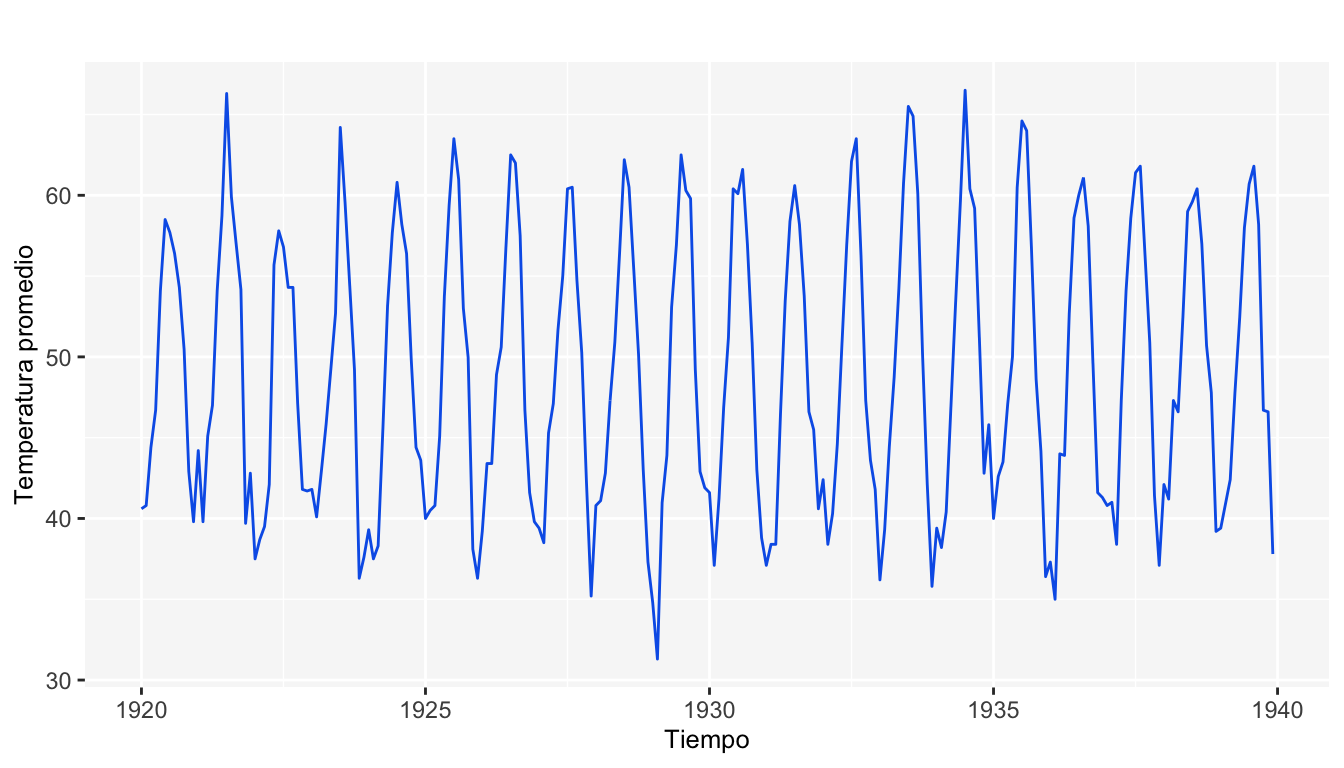
\includegraphics{_main_files/figure-latex/unnamed-chunk-6-1} \end{center}

La función R ``decompose'', obtiene las componentes de tendencia, estacionalidad y aleatoria de una serie temporal a través de medias móviles, y además permite obtener los componentes en base a un esquema aditivo ó multiplicativo. Es una función generica de R, lo que significa que no requiere de la instalación de ninguna librería.

Las siguientes gráficas representan las componentes antes mencionadas de esta serie de tiempo.

\begin{center}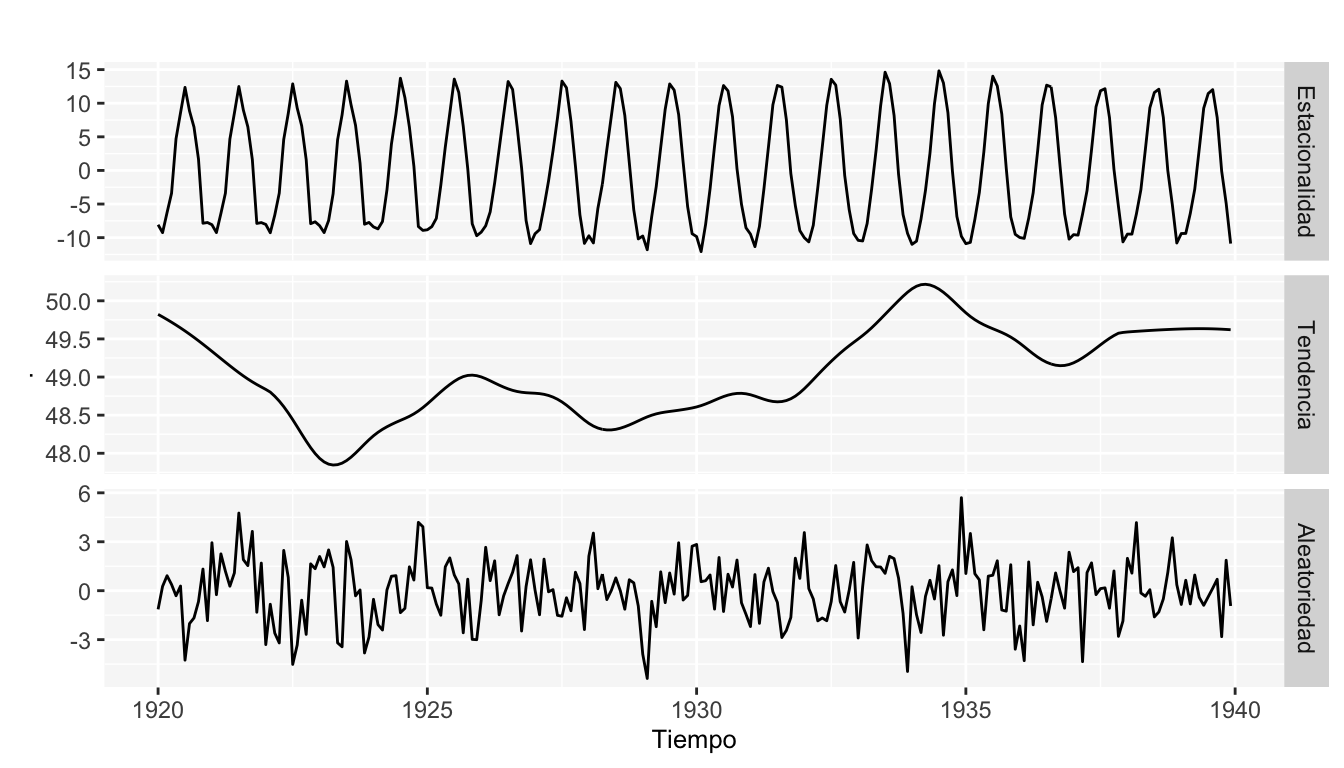
\includegraphics{_main_files/figure-latex/unnamed-chunk-7-1} \end{center}

Según las características de las series de tiempo estas pueden clasificarse en:

\textbf{Estacionarias}: Una serie de tiempo estacionaria es estable a lo largo del tiempo, es decir su media, varianza y \textbf{autocovarianza} (en diferentes rezagos o diferentes tiempos) son constantes en el tiempo.

Es decir que sin importar el momento en que se midan (invariantes respecto al tiempo) se debe cumplir lo siguiente:

\begin{itemize}
\tightlist
\item
  Media: \(\mathbb{E}(X_t) = \mathbb{E}(X_{t+k}) = \mu\)
\item
  Varianza: \(Var(X_t) = Var(X_{t+k}) = \sigma^2\)
\item
  Covarianza: \(\mathbb{E}[(X_t-\mu)(X_{t+k}-\mu)] = \gamma_k\)
\end{itemize}

Aquí se muestra un ejemplo en el cual la varianza no cambia a lo largo del tiempo y la media permanece constante

\begin{center}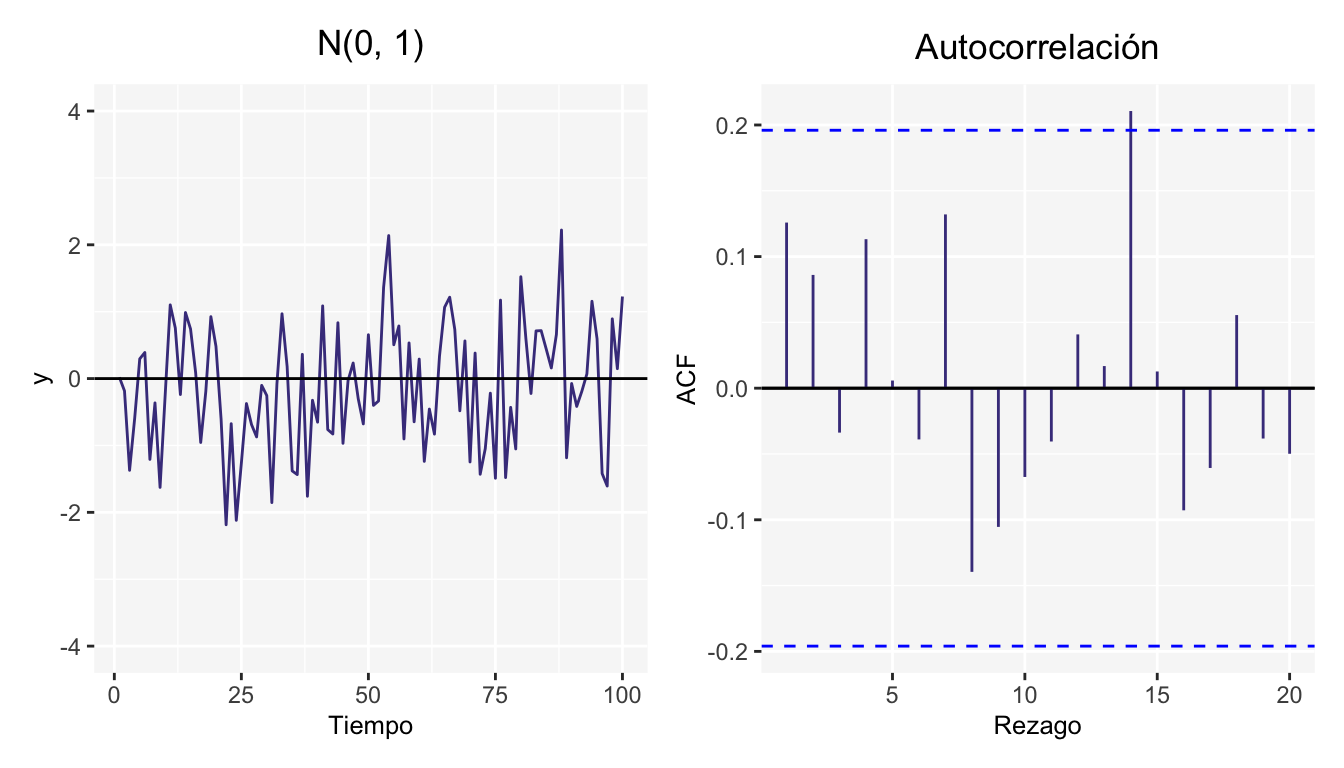
\includegraphics{_main_files/figure-latex/unnamed-chunk-8-1} \end{center}

\textbf{No estacionaria}: Son series en las cuales la tendencia y/o variabilidad cambian en el tiempo. Los cambios en la media determinan una tendencia a crecer o decrecer a largo plazo, por lo que la serie no oscila alrededor de un valor constante. Existen muchos casos en este tipo de series, aquí se muestran algunos ejemplos.

\begin{center}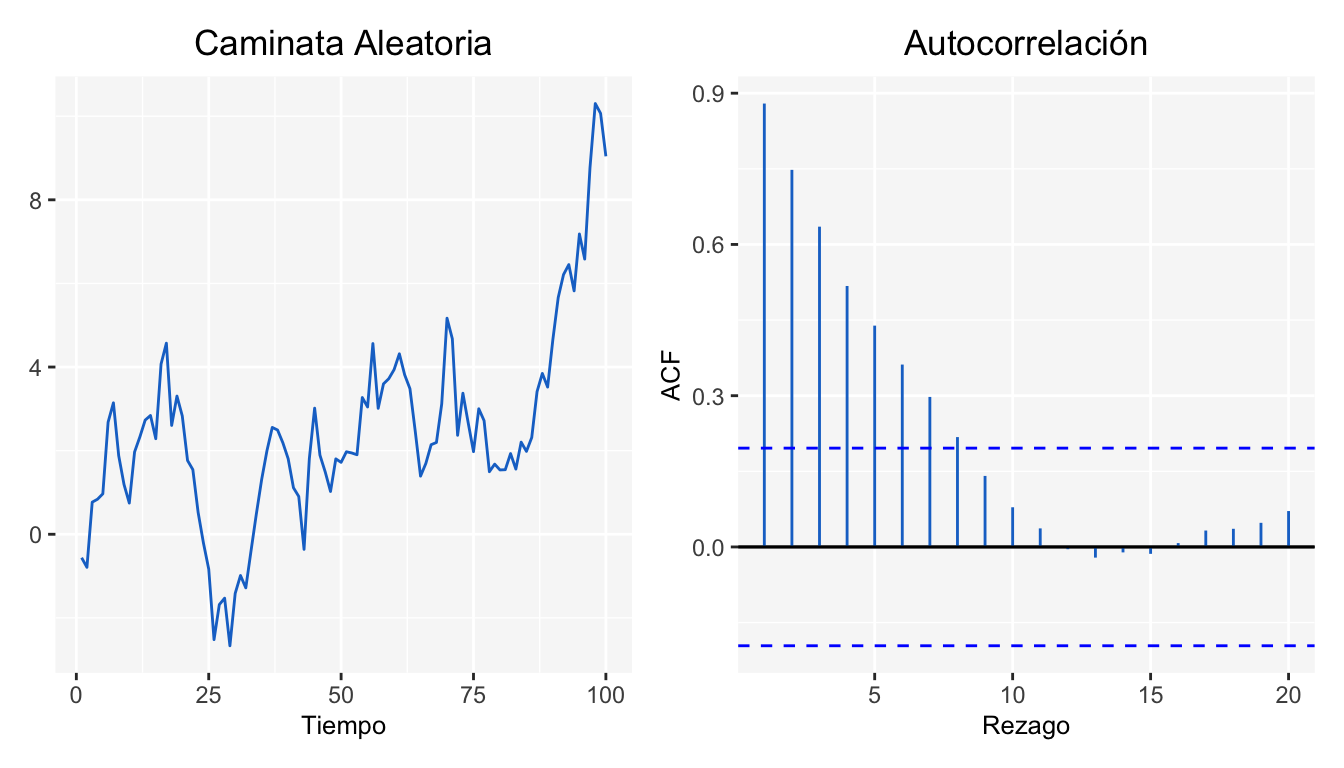
\includegraphics{_main_files/figure-latex/unnamed-chunk-9-1} \end{center}

\hypertarget{procesos-estocuxe1sticos}{%
\chapter{Procesos estocásticos}\label{procesos-estocuxe1sticos}}

La palabra estocástico, que tiene origen Griego, era usada bajo el significado de \emph{perteneciente al azar}. En ese sentido un proceso estocástico se define como un conjunto de variables aleatorias ordenadas según el tiempo (o el espacio que corresponda), el cual puede ser continuo o discreto.
Se denota la variable aleatoria en el tiempo \(t\) por \(X(t)\) o \(X_t\) con \(-\infty < t < \infty\) en caso de ser continua o bien \(t = (0, \pm1, \pm2, ... )\) en caso de ser discreta.

Como un ejemplo de proceso estocástico tenemos, el número de personas que esperan en una fila en el instante \(t\) del tiempo.

\hypertarget{proceso-estocuxe1stico-estacionario}{%
\section{Proceso estocástico estacionario}\label{proceso-estocuxe1stico-estacionario}}

Al trabajar con series de tiempo el escenario ideal sería trabajar con series que posean la característica de tener la media y la autocovarianza constantes a lo largo del tiempo, es decir, que sus valores oscilen dentro de un rango de valores y no muestren tendencia clara, creciente o decreciente, teóricamente conocidos como procesos estacionarios. Para definir un proceso estocástico como un proceso estacionario es sumamente necesario conocer la función de densidad conjunta de las variables aleatorias que conforman el proceso, no obstante, en la práctica no es común que se logre. Es por esto por lo que los procesos estacionarios se pueden definir de la siguiente forma:

\begin{itemize}
\item
  \textbf{Procesos estrictamente estacionarios:} Se dice que un proceso \(X_t, t \in Z\) es estrictamente estacionario, si sus funciones de densidad para un conjunto arbitrario de variables \(X_t,X_{t+1}, ... , X_{t+m}\) son invariantes respecto a desplazamientos en el tiempo, es decir, que cumplen:
  \[
  \begin{array}{cc}
  f(X_t,X_{t+1}, ... , X_{t+m}) = f(X_{t+k}, X_{t+k+1}, ... , X_{t+k+m}) & \forall t, m, k \in Z
  \end{array}
  \]
\item
  \textbf{Procesos débilmente estacionarios:} Un proceso \(X_t,t\in Z\) se dice que es débilmente estacionario de orden \(k\) si los primeros \(k\) momentos son invariantes a través del tiempo. Podemos definir un proceso débilmente estacionario de segundo orden si cumple lo siguiente:

  \begin{enumerate}
  \def\labelenumi{\arabic{enumi}.}
  \tightlist
  \item
    \(E\left[|X_t|^2\right]< \infty \forall t \in Z\)
  \item
    \(E[X_t] = \mu \ \ \forall t \in Z\), lo cual quiere decir que las esperanzas de las variables aleatorias son independientes del tiempo por lo cual permanecen constantes.
  \item
    \(Cov(X_t,X_s) = Cov (X_{t+m}, X_{s+m}) \forall t, s, m \in Z\), es decir las covarianzas de dos variables aleatorias del proceso que se encuentran en distintos puntos del tiempo dependen solamente del lapso transcurrido entre cada una de ellas.
  \end{enumerate}
\end{itemize}

En resumen, si una serie es estacionaria, su media, su varianza y su autocovarianza (en diferentes rezagos) permanecen iguales sin importar el momento en el cual se midan; es decir, son invariantes respecto al tiempo.

\hypertarget{ruido-blanco-white-noise}{%
\section{Ruido blanco (``white noise'')}\label{ruido-blanco-white-noise}}

Un ruido blanco\footnote{El nombre de ruido blanco puede explicarse fácilmente en el análisis espectral en series de tiempo, el cual hace un estudio sobre la frecuencia y no tanto sobre el tiempo. Este no se verá en este material pero se puede estudiar a detalle esto en el libro \citet{cryer2008time}. Bajo un análisis espectral, en un proceso de ruido, su función de densidad espectral (se puede pensar la densidad espectral como la cantidad de varianza en un intervalo \((\omega, \omega+d\omega)\) que aporta un modelo basado en una serie de Fourier) es constante, es decir que esto sucede para todas las frecuencias. Esto es análogo al espectro de luz blanca en el ámbito físico; ya que todos los colores se distribuyen uniformemente para formar la luz blanca.} es un caso simple de los procesos estocásticos, donde los valores son independientes e idénticamente distribuidos a lo largo del tiempo con media cero e igual varianza, se denota por \(\epsilon_t\).
\[
\begin{array}{c}
\epsilon_t \sim N(0,\sigma^2)\\
Cov(\epsilon_{t_i},\epsilon_{t_j})=0 \space \forall t_i \neq t_j
\end{array}
\]

\begin{center}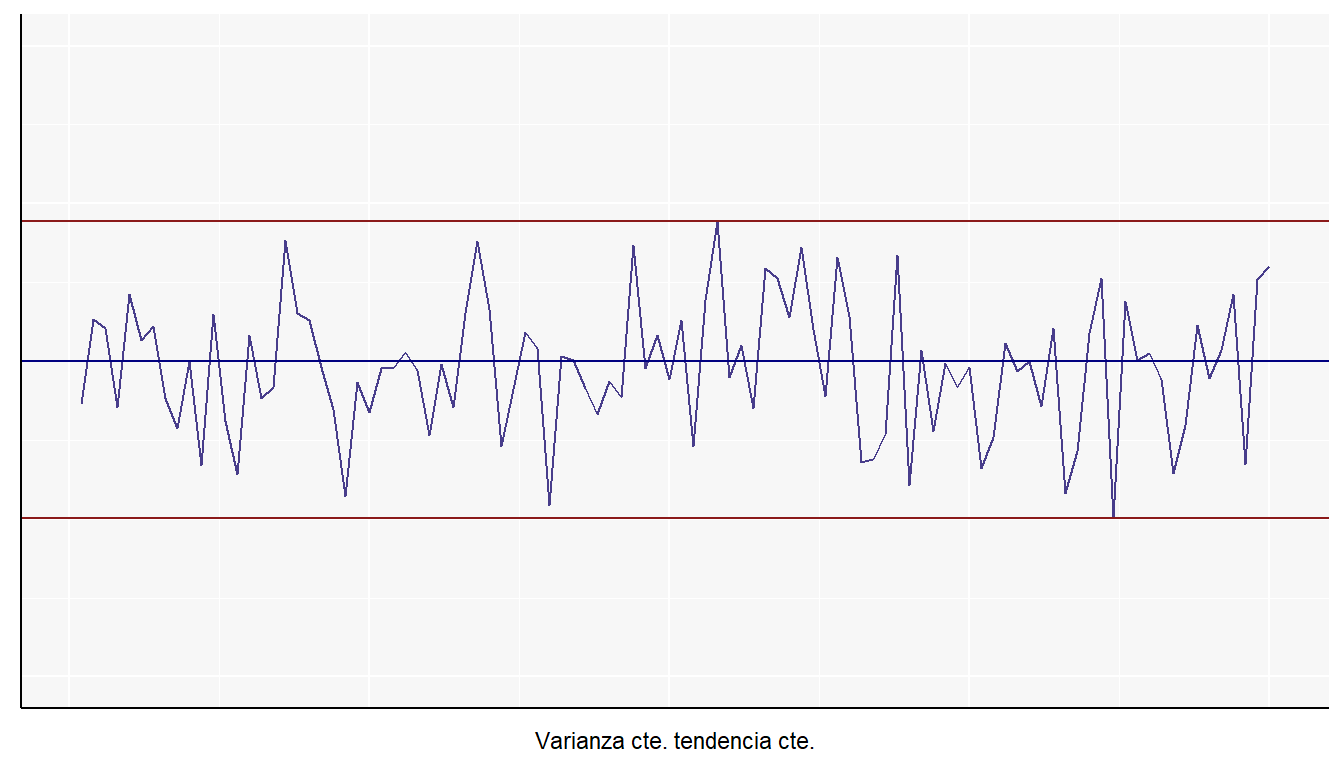
\includegraphics{_main_files/figure-latex/unnamed-chunk-10-1} \end{center}

La segunda gráfica lleva el nombre de \textbf{correlograma}, la cual esta creada con los valores de autocorrelación, los cuales se ven en el siguiente capítulo.

\hypertarget{caminata-aleatoria}{%
\section{Caminata aleatoria}\label{caminata-aleatoria}}

Es un proceso estocástico \(X_t\) donde la primera diferencia de este proceso es un ruido blanco: \(\nabla X_{t} = \epsilon_t\)

\begin{center}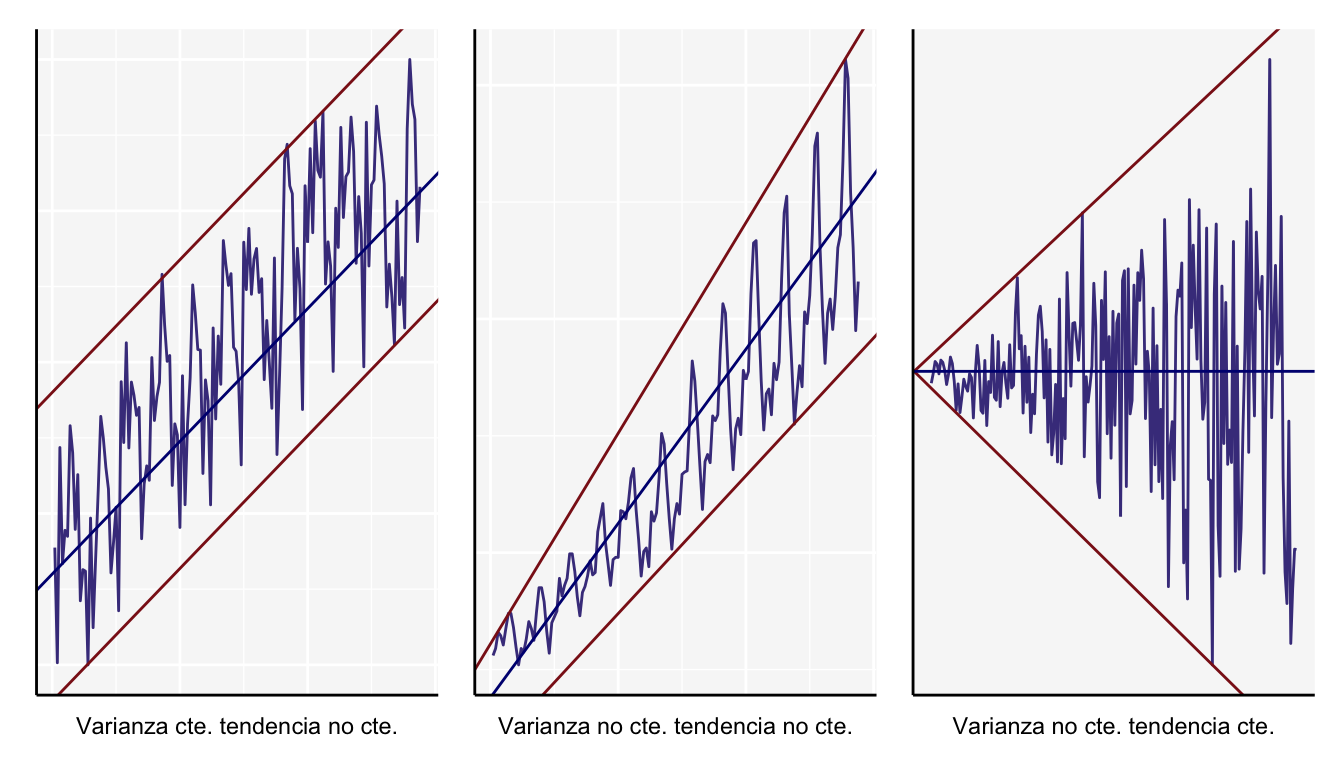
\includegraphics{_main_files/figure-latex/unnamed-chunk-11-1} \end{center}

La anterior gráfica esta basada en 100 simulaciones de una normal estándar bajo con una semilla en 123.

\hypertarget{ejercicios}{%
\subsection{Ejercicios}\label{ejercicios}}

\begin{enumerate}
\def\labelenumi{\arabic{enumi})}
\tightlist
\item
  Reproducir la caminata aleatoria con semilla (123) mostrada en la gráfica anterior.
\item
  Ver ¿qué sucede al aumentar el número de simulaciones \((n=1000)\)? ¿Por qué sucede este nuevo comportamiento?
\end{enumerate}

\hypertarget{funciones-de-autocovarianza-y-autocorrelaciuxf3n}{%
\chapter{Funciones de autocovarianza y autocorrelación}\label{funciones-de-autocovarianza-y-autocorrelaciuxf3n}}

Como se mencionó en el apartado anterior, tenemos que para un proceso estacionario \(X_t\), su esperanza es \(E[X_t] = \mu\) y su varianza \(Var[X_t]=E[X_t-\mu]^2=\sigma^2\) las cuales son constantes; así como las covarianzas \(Cov(X_t,X_s)\), que son funciones que solamente dependen del tiempo que transcurre entre \(t\) y \(s\); entonces en este caso podemos escribir la \textbf{covarianza} entre \(X_t\) y \(X_{t+k}\) como:

\[
\gamma_k=Cov(X_t,X_{t+k})=E(X_t-\mu)(X_{t+k}-\mu)
\]

Y su \textbf{correlación} como:
\[
\rho_k =\frac{Cov(X_t,X_{t+k})}{\sqrt{Var(X_t)}\sqrt{Var(X_{t+k})}}=\frac{\gamma_k}{\gamma_0}
\]

donde, \(Var(X_t) = Var(X_{t+k}) = \gamma_0\).

También conocida como la \textbf{función de autocorrelación (ACF)}, la cual es una medida de la relación para los valores de la serie respecto a los valores de esta misma, observados \(k-t\) unidades de tiempo.

La función de autocorrelación tiene las siguientes propiedades:

\begin{itemize}
\tightlist
\item
  \(\rho_0=1\)
\item
  \(-1\leq\rho_j\leq 1\)
\item
  \(\rho_j=\rho_{-j}\)
\end{itemize}

En general, se utiliza la función de autocorrelación muestral \(r_k\), la cual queda determinada por la siguiente expresión

\[
r_k=\frac{\sum\limits_{t = k+1}^n (X_t-\bar{X})(X_{t-k}-\bar{X})}{\sum\limits_{t = 1}^n(X_t-\bar{X})^2}
\]

Para \(k = 1, 2, \dots\) y donde \(\bar{X}\) es la media de las observaciones.

\hypertarget{funciuxf3n-de-autocorrelaciuxf3n-parcial}{%
\section{Función de autocorrelación parcial}\label{funciuxf3n-de-autocorrelaciuxf3n-parcial}}

La función de correlación parcial estima la correlación entre una observación \(k\) tiempos después de la observación actual removiendo los efectos de las correlaciones de las observaciones intermedias; es decir:

\[
\pi_j=corr(X_j,X_{j-k}|X_{j-1},X_{j-2},...X_{j-k-1})
\]

Para este caso, el estimador apropiado es la función de autocorrelación parcial muestral \citet{cryer2008time}, el cual puede obtenerse utilizando \(r_k\) para la siguiente expresión recursiva.

\[
\pi_j=\frac{\rho_j-\sum\limits_{k = 1}^{j-1}\pi_{j-1, k}\rho_{j-k}}{1-\sum\limits_{k = 1}^{j-1}\pi_{j-1, k}\rho_k}
\]
donde \(\pi_{j, k} = \pi_{j-1, k}-\pi_{j}\pi_{j-1, j-k}\) para \(k = 1,2, \dots, j-1\).

\hypertarget{correlograma}{%
\section{Correlograma}\label{correlograma}}

Una vez calculadas las funciones de autocorrelación y autocorrelación parcial, se grafican contra los diferentes rezagos para obtener los correlogramas. Estos son serán de gran utilidad para la identificación del modelo, tal como se menciona en el capítulo \ref{modelacion-univariada} y en el complemento a este material \href{https://rpubs.com/CarlosFVG/SeriesTCodeCFVG}{SeriesTCode}. Como ejemplo, se presentan los gráficos correspondientes a los datos de \texttt{nottem}.

\begin{center}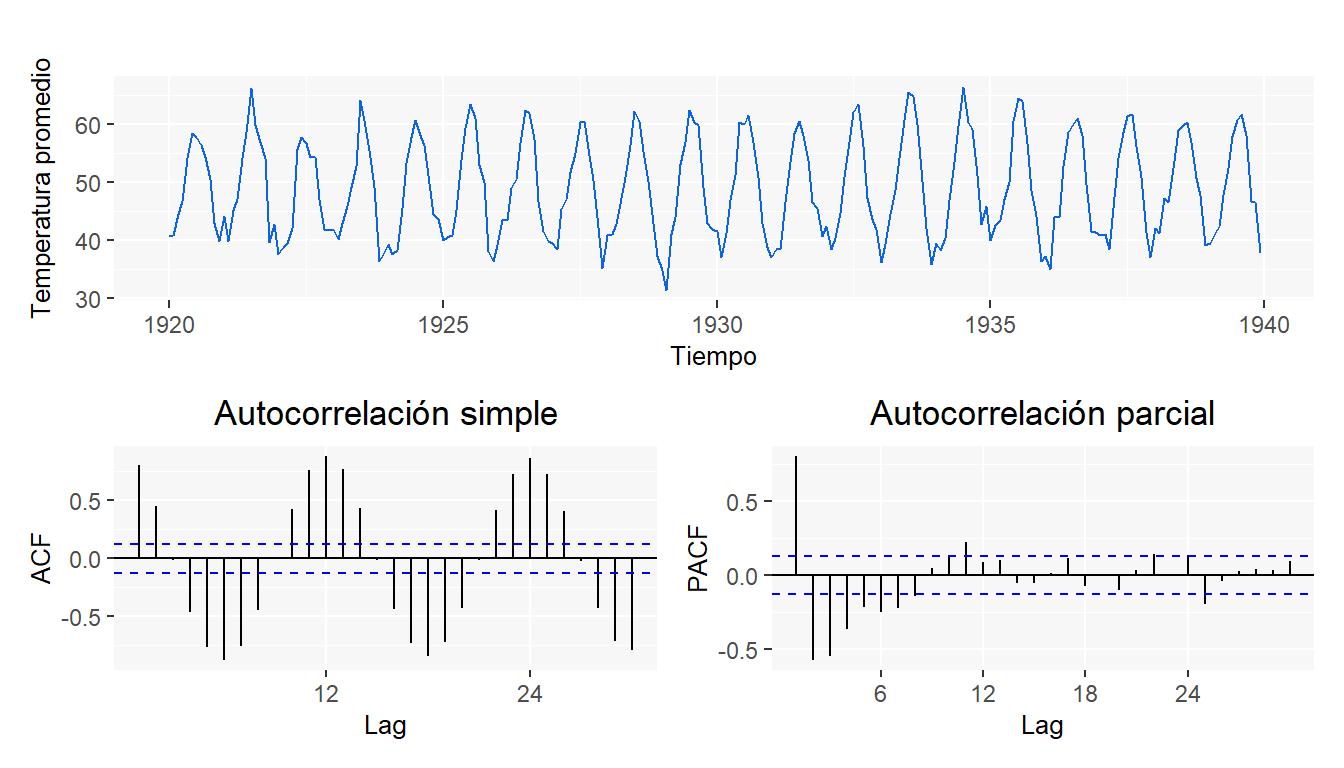
\includegraphics{_main_files/figure-latex/unnamed-chunk-12-1} \end{center}

\hypertarget{prueba-de-ljung-box}{%
\section{Prueba de Ljung-Box}\label{prueba-de-ljung-box}}

Esta prueba permite probar en forma conjunta que todos los coeficientes de autocorrelación son simultáneamente iguales a cero. La prueba está definida como

\[
LB=n(n+2)\sum_{k=1}^m\frac{\hat\rho_k^2}{n-k}\sim \chi_{(m)}^2
\]
donde \(n\) es el tamaño de la muestra, \(m\) la longitud del rezago.

Las hipótesis de esta prueba son:

\[
\begin{array}{cc}
H_0:\mbox{Los coeficientes de autocorrelación son simultáneamente iguales a cero}\\
H_1: \mbox{Alguno de los coeficientes de autocorrelación es distinto de cero}
\end{array}
\]

Entonces si \(LB\) excede el valor crítico de la tabla \(Ji\) cuadrada al nivel de significancia seleccionado, no se acepta la hipótesis de que todos los coeficientes de autocorrelación son iguales a cero, por lo tanto al menos algunos de ellos deben ser diferentes de cero\footnote{Originalmente la prueba esta diseñada para comprobar estadísticamente si las observaciones son independientes entre sí, bajo esta hipótesis, los coeficientes de correlación serán cero y el estadístico \(LB\) será cercano a cero. Esta prueba es de gran ayuda para ver la calidad del modelo que se aplique y para validar las hipótesis que se puedan requerir en la construcción de intervalos de predicción. Se hablará más de su uso en el capítulo \ref{modelacion-univariada}.}.

\hypertarget{transformaciones}{%
\chapter{Transformaciones}\label{transformaciones}}

La mayoría de las series de tiempo no son débilmente estacionarias, es decir que no muestran una media ni una varianza constantes a lo largo del tiempo y pueden mostrar tendencias crecientes o bien, decrecientes. Para poder trabajar con este tipo de series de una forma más sencilla y manejable, existen métodos para transformarlas y verlas como realizaciones de una serie de tiempo débilmente estacionaria. Las transformaciones más comunes son el suavizamiento a través de medias móviles o ajustando polinomios a la serie en cuestión, la diferenciación.

\hypertarget{suavizamiento-por-medias-muxf3viles}{%
\section{Suavizamiento por medias móviles}\label{suavizamiento-por-medias-muxf3viles}}

Se mencionó que las series de tiempo se pueden ver como la suma de tres componentes: una tendencia, una estacionalidad y una componente aleatorio o irregular. Ahora bien, en este método de suavizamiento el objetivo es estimar y extraer \textbf{la tendencia} \(\left(T_t\right)\) del modelo. Lo anterior se puede realizar estimando la tendencia con:

\[
\hat T_t=(2q+1)^{-1}\sum_{j=-q}^q X_{t-j},\space q+1\leq t\leq n-q
\]

Este es uno de mucho filtros lineales que podrían aplicarse (\(\hat T_t=\sum_{j=-\infty}^\infty a_jX_{t-j}\)). Obsérvese que para valores grandes de \(q\), \((2q+1)^{-1}\sum_{j=-q}^q [X_{t-j}-\hat T_t]\approx 0\), lo cual no sólo atenua el ruido, también permite que la tendencia lineal \(T_t=c_0+c_1t\) pase sin distorsión. Sin embargo hay que tener cuidado en la selección de \(q\), ya que valores muy grandes, si \(T_t\) no es lineal, entonces se suavizará la serie pero la estimación de la tendencia será mala.

\hypertarget{suavizamiento-por-polinomios-ajustados}{%
\section{Suavizamiento por polinomios ajustados}\label{suavizamiento-por-polinomios-ajustados}}

En este método de suavizamiento el objetivo es estimar y extraer la \textbf{tendencia} (\(T_t\)) y la \textbf{estacionalidad} (\(E_t\)) del modelo. Si \(E_t= 0\), se tiene un caso de no estacionariedad simple, por lo que el proceso tiene un comportamiento estacionario alrededor de la tendencia y para estimar \(T_t\) se supone que tiene la siguiente forma:

\[
T_t = a_0 + a_1t +... + a_pt^p
\]

Si se tiene \(p = 1\) la tendencia es lineal, si \(p = 2\) la tendencia es cuadrática.

Los parámetros \(a_i\) se estiman mediante mínimos cuadrados ordinarios, es decir que minimicen \(\sum_{i=1}^n (x_i-T_i)^2\).

\hypertarget{diferencias-de-box-jenkins}{%
\section{Diferencias de Box-Jenkins}\label{diferencias-de-box-jenkins}}

Consiste en aplicar diferencias a la serie de tiempo estudiada hasta que las observaciones se perciban como componentes de una serie débilmente estacionaria. Se debe comprender los siguientes operadores para el método:

El \textbf{operador de retraso} se denota con una letra \(B\) o \(\mathcal{L}\) y se define como el valor retrasado de una serie de tiempo temporal indicado por el exponente del operador. De manera particular se tiene \(BX_t = X_{t-1}\), por lo que si se aplica varias veces el operador, la serie se retardaría \(k\)-unidades temporales:

\[
B^kX_t=X_{t-k}
\]

En particular \(B^0X_t=X_t\). Se puede utilizar con notación polinómica:

\[
\phi(B)X_t = \left(\phi_0+\phi_1B+\phi_2B^2\right)X_t = \phi_0X_t+\phi_1X_{t-1}+\phi_2X_{t-2} 
\]

El \textbf{operador diferencia} se expresa con \(\nabla\) y se define como la diferencia entre el valor al periodo \(t\) y valor rezagado \(k\) periodos \(\nabla X_t=X_t-X_{t-1}\).

Ambos operadores se relacionan de la siguiente manera:

\[
\nabla Z_t=Z_t-Z_{t-1}=Z_t-BZ_t=(1-B)Z_t
\]
Teniendo que \(\nabla=(1-B)\)

Si aplicamos el operador diferencia sucesivamente entonces se obtiene:

\[
\begin{array}{cc}
\nabla^k=(1-B)^k; & \nabla^kX_t=\sum_{j=0}^k\frac{k!}{j!(k-j)!}(-1)^jX_{t-j}
\end{array}
\]

\hypertarget{part-procesos-lineales-estacionarios}{%
\part{Procesos lineales estacionarios}\label{part-procesos-lineales-estacionarios}}

\hypertarget{arp-proceso-autoregresivo}{%
\chapter{\texorpdfstring{\(AR(p)\): Proceso Autoregresivo}{AR(p): Proceso Autoregresivo}}\label{arp-proceso-autoregresivo}}

Los modelos autoregresivos se basan en la idea de que el valor actual de la serie \(X_t\), puede explicarse en función de \(p\) valores pasados \(X_{t-1},X_{t-2},...X_{t-p}\), donde \(p\) determina el número de rezagos necesarios para pronosticar un valor actual.

El modelo autoregresivo de orden \(p\) está dado por:

\[
X_t=\phi_0+\phi_1X_{t-1}+\phi_2X_{t-2}+...+\phi_pX_{t-p}+\epsilon_t
\]

Expresado en términos del operador de retardos

\[
X_t-\phi_0-\phi_1X_{t-1}-\phi_2X_{t-2}-...-\phi_pX_{t-p}=\epsilon_t
\\-\phi_0+(1-\phi_1B-\phi_2B^2-\phi_3B^3-...-\phi_pB^p)X_t=\epsilon_t
\\\phi_p(B)X_t=\epsilon_t+\phi_0
\]

donde \(\epsilon_t\) es un proceso de ruido blanco y \(\phi_0,\phi_1,\phi_2,...\phi_p\) son parámetros del modelo.

\hypertarget{proceso-autoregresivo-de-orden-1-ar1}{%
\section{\texorpdfstring{Proceso Autoregresivo de orden 1: \(AR(1)\)}{Proceso Autoregresivo de orden 1: AR(1)}}\label{proceso-autoregresivo-de-orden-1-ar1}}

En los procesos \(AR(1)\) la variable \(X_t\) está determinada únicamente por el valor pasado, esto es \(X_{t-1}\).

\[
X_t=\phi_0+\phi_1X_{t-1}+\epsilon_t
\]

Donde \(\epsilon_t\) es un ruido blanco con media \(0\) y con varianza \(\sigma^2\) e independiente de \(X_t\). Para verificar que sea estacionario (débilmente) se debe verificar la estacionalidad en media y covarianza.

\hypertarget{estacionario-en-media}{%
\subsection{Estacionario en Media}\label{estacionario-en-media}}

\[
\begin{split}
\mathbb{E}(X_t) &= \mathbb{E}(\phi_0+\phi_1X_{t-1}+ \epsilon_t)= \phi_0 + \phi_1 \mathbb{E}(X_{t-1}) + \mathbb{E}(\epsilon_t)\\
& = \phi_0 + \phi_1\mathbb{E}(X_{t-1})\\
\end{split}
\]
Para que \(X_t\) sea estacionario en la media se debe cumplir que \(E(X_t)=E(X_{t-1})\)

Entonces:

\[
(1-\phi_1)\mathbb{E}(X_t)=\phi_0   \       \       \Longrightarrow \  \ E(X_t)= \frac {\phi_0}{1-\phi_1} 
\]
por lo tanto \(E(X_t)=\frac {\phi_0}{1-\phi_1}\) y \(\phi_1\neq1\).

\hypertarget{estacionario-en-covarianza}{%
\subsection{Estacionario en Covarianza}\label{estacionario-en-covarianza}}

Para que \(AR(1)\) sea estacionario, la varianza tiene que ser constante y finita en el tiempo.

\[
\begin{split}
\gamma_0 &= Var(X_t)=\mathbb{E} \left[(X_t -\mathbb{E}(X_t))^{2}\right]\\
&= \mathbb{E}\left[(\phi_0+\phi_1X_{t-1}+\epsilon_t-\phi_0-\phi_1\mathbb{E}(X_{t-1}))^2\right]\\
& = \mathbb{E}\left[(\phi_1(X_{t-1}-\mathbb{E}(X_{t-1}))+\epsilon_t)^2\right]\\
& = \mathbb{E}\left[\phi_1(X_{t-1}-\mathbb{E}(X_{t-1}))^2+2\phi_1(X_{t-1}-\mathbb{E}(X_{t-1}))\epsilon_t+\epsilon_t^2\right]\\
& = \phi^2 \mathbb{E}\left[(X_{t-1}-\mathbb{E}(X_{t-1}))^2\right] +2\phi_1\mathbb{E}\left[X_{t-1}-\mathbb{E}(X_{t-1})\right]\mathbb{E}(\epsilon_t)+\mathbb{E}[\epsilon_t^2]\\
&= \phi_1^2 Var(X_{t-1})+ \sigma^2
\end{split}
\]

Buscamos que \(X_t\) sea estacionario en la varianza, por lo que bajo el supuesto de proceso estacionario:

\[
\begin{split}
&\Longrightarrow  Var(X_t)=Var(X_{t-1})\\
&\Longrightarrow  Var(X_t)= \gamma_0= \phi_1^2 Var(X_{t-1})+\sigma^2\\
&\Longrightarrow \gamma_0=\phi_1^2 \gamma_0+ \sigma^2 \Longrightarrow (1-\phi_1^2) \gamma_0=\sigma^2\\
&\Longrightarrow \gamma_0 = \frac{\sigma^2}{1-\phi_1^2}
\end{split}
\]

Véase que para que sea estacionario, con varianza constante y finita es necesario que \(| \phi_1|< 1\). En resumen

\[Var(X_t)= \gamma_0 = \frac{\sigma^2}{1-\phi^2}\]

Respecto a la covarianza \(Cov(X_t,X_{t-k})\) para \(K=1,...\), se tiene lo siguiente

\[
\begin{split}
Cov(X_t,X_{t-k})&=\gamma_k = \mathbb{E}\left[(X_t-\mathbb{E}(X_t))(X_{t-k}-\mathbb{E}(X_{t-k}))\right]\\
& = \mathbb{E}\left[(\phi_1(X_{t-1}-\mathbb{E}(X_{t-1}))+\epsilon_t)(X_{t-k}-\mathbb{E}(X_{t-k}))\right]\\
& = \mathbb{E}\left[\phi_1(X_{t-1}-\mathbb{E}(X_{t-1}))(X_{t-k}-\mathbb{E}(X_{t-k}))\right] + \mathbb{E}\left[\epsilon_t(X_{t-k}-\mathbb{E}(X_{t-k}))\right]\\
& = \phi_1\mathbb{E}\left[(X_{t-1}-\mathbb{E}(X_{t-1}))(X_{t-k}-\mathbb{E}(X_{t-k}))\right] = \phi_1\gamma_{k-1}
\end{split}
\]

\[
\begin{array}{lc}
\mbox{Entonces: } & 
\begin{array}{c}
\gamma_1= \gamma_0 \phi\\
\gamma_2 =\gamma_1\phi\\
\vdots
\end{array}
\end{array}
\]

\(\therefore AR(1)\) es estacionario en covarianza si \(|\phi_1|<1\) y la \textbf{función de covarianza} será:

\[
\gamma_k=
\left\{
\begin{aligned}
\frac{\sigma^2}{1-\phi_1^2} \ \ \   \  k=0\\
\phi_1 \gamma_{k-1} \ \ \ \ k>0
\end{aligned}
\right.
\]

Los \textbf{coeficientes de correlación} quedan determinados por la siguiente expresión:

\[
\rho_k = \frac{Cov(X_t, X_{t-k})}{\sqrt{Var(X_t)}\sqrt{Var(X_{t-k})}} = \frac{\gamma_k}{\gamma_0} = \frac{\phi_1\gamma_{k-1}}{\gamma_0} = \phi_1\frac{\gamma_{k-1}}{\gamma_0} = \phi_1\rho_{k-1}
\]

Por lo que la \textbf{función de autocorrelación} para \(AR(1)\) es :

\[
\rho_k=
\left\{
\begin{aligned}
 1  \ \ \ \ \ \ k=0\\
\phi \rho_{k-1} \ \ \ \ k\geq 1
\end{aligned}
\right.
= 
\left\{
\begin{array}{lr}
1 &  k=0\\
\phi_1\frac{\gamma_{k-1}}{\gamma_o} & k\geq 1
\end{array}
\right.
\]

Observemos que para el modelo \(AR(1)\), la función de autocorrelación es exponencial

\[
\begin{split}
\rho_0 &= 1\\
\rho_1&=\phi_1\rho_o=\phi_1\\
\rho_2&=\phi_1\rho_1=\phi_1^2\\
&\ \ \vdots\\
\rho_k&=\phi_1^k
\end{split}
\implies
\rho_k=
\left\{
\begin{array}{lr}
 1  & k=0\\
\phi_1^2 & k\geq 1
\end{array}
\right.
\]

\begin{itemize}
\tightlist
\item
  Caso particular: \(AR(1): X_t = \phi_1X_{t-1}+\epsilon_t\), es decir que \(\phi_0 = 0\). Para este caso se tiene \(\mathbb{E}(X_t) = \phi_1\mathbb{E}(X_{t-1})\implies(1-\phi_1)\mathbb{E}(X_t) = 0\implies\mathbb{E}(X_t) = \frac{0}{(1-\phi_1)} = 0\).
\end{itemize}

A continuación se muestran los resultados para un modelo \(AR(1)\) de la siguiente forma \(X_t=0.35X_{t-1}+\epsilon_t\)

\begin{center}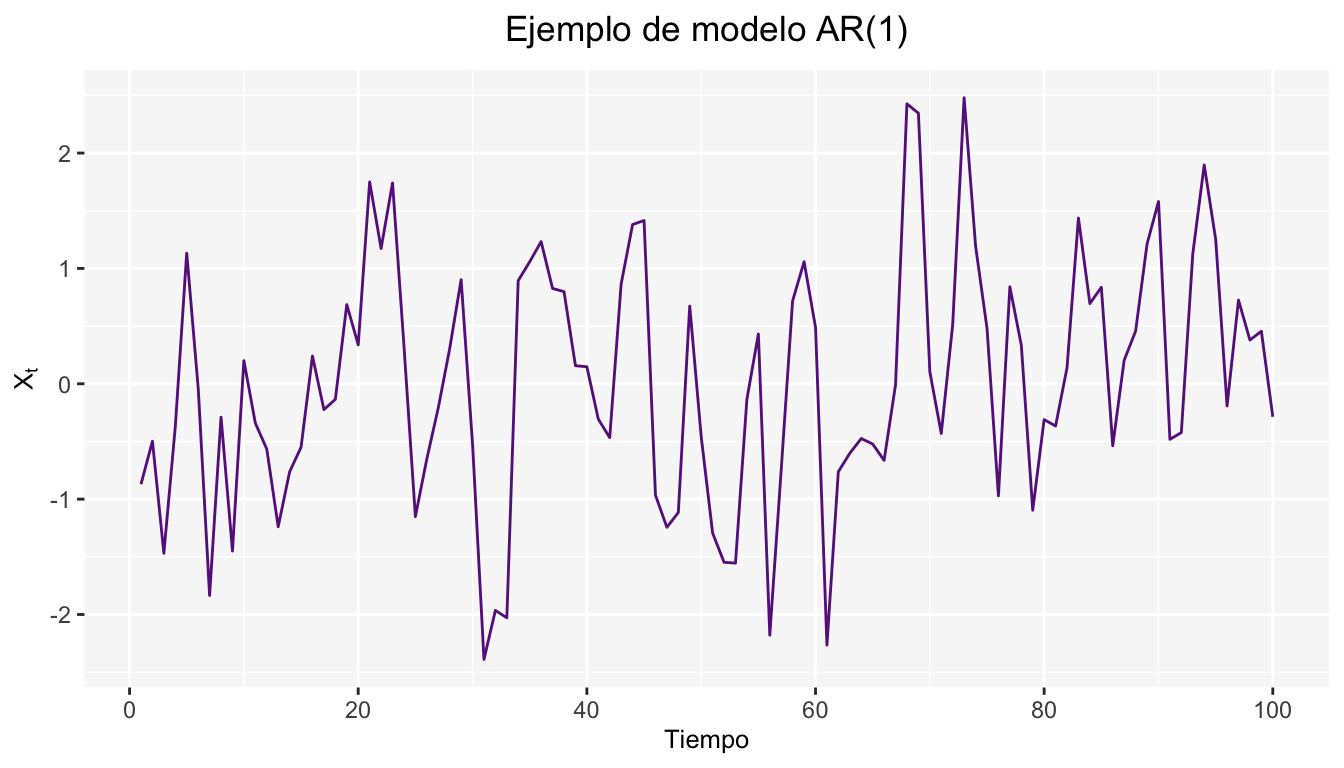
\includegraphics{_main_files/figure-latex/unnamed-chunk-13-1} \end{center}

Además de las gráficas de Autocorrelación simple y parcial.

\begin{center}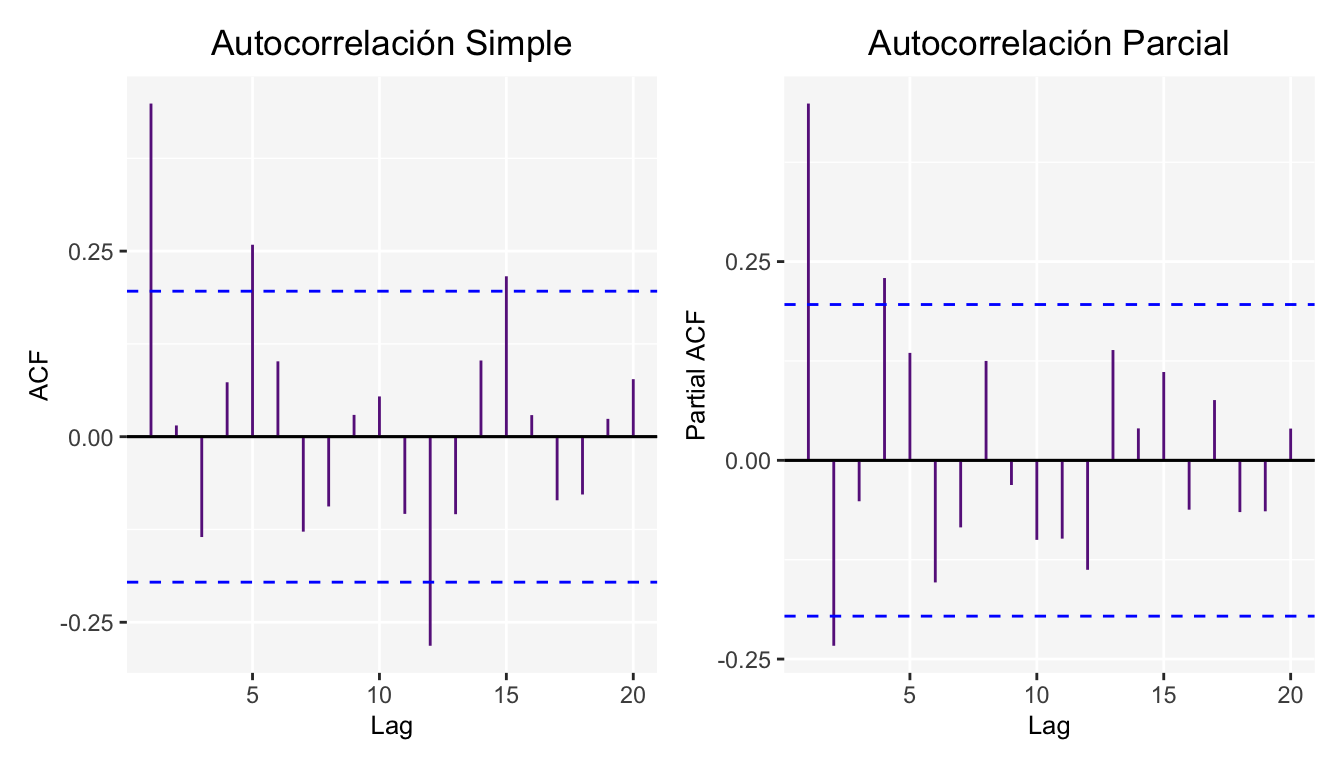
\includegraphics{_main_files/figure-latex/unnamed-chunk-14-1} \end{center}

\hypertarget{proceso-autoregresivo-de-orden-2-ar2}{%
\section{\texorpdfstring{Proceso Autoregresivo de orden 2: \(AR(2)\)}{Proceso Autoregresivo de orden 2: AR(2)}}\label{proceso-autoregresivo-de-orden-2-ar2}}

En los procesos \(AR(2)\) la variable \(X_t\) está determinada por el valor pasado y el anterior a este.

\[
X_t=\phi_0 + \phi_1 X_{t-1}+\phi_2 X_{t-2}+\epsilon_t
\]

Donde \(\epsilon_t\) es un ruido blanco (media cero y varianza \(\sigma^2\)). Asumiendo estacionariedad débil, se tiene que la media y la varianza del proceso serán las siguientes.

\hypertarget{estacionario-en-media-1}{%
\subsection{Estacionario en Media}\label{estacionario-en-media-1}}

Bajo el supuesto de estacionalidad:

\[
\begin{split}
& \mathbb{E}(X_t) = \mathbb{E}(X_{t-1}) = \mathbb{E}(X_{t-2})\\
\implies &(1-\phi_1-\phi_2)\mathbb{E}(X_t) = \phi_0\\
\implies &\mathbb{E}(X_t) = \frac{\phi_0}{1-\phi_1-\phi_2}
\end{split}
\]

\(\therefore\) Para que sea estacionario, se tiene que cumplir que \(1-\phi_1-\phi_2 \neq 0\).

\hypertarget{estacionario-en-covarianza-1}{%
\subsection{Estacionario en Covarianza}\label{estacionario-en-covarianza-1}}

\[
\begin{split}
\gamma_0 &= \mathbb{E}\left[(X_t-\mathbb{E}(X_t))^2\right]\\
& = \mathbb{E}\left[(\phi_0+\phi_1 X_{t-1}+\phi_2 X_{t-2}+\epsilon_t-\phi_0 -\phi_1\mathbb{E}(X_{t-1})-\phi_2 \mathbb{E}(X_{t-2}))^2\right]\\
& = \mathbb{E}\left[(\phi_1(X_{t-1}-\mathbb{E}(X_{t-1}))+\phi_2(X_{t-2}-\mathbb{E}(X_{t-2}))+\epsilon_0)^2\right]\\
& = \mathbb{E}[\phi_1^2(X_{t-1}-\mathbb{E}(X_{t-1}))^2 + 2\phi_1\phi_2(X_{t-1}-\mathbb{E}(X_{t-1}))(X_{t-2}-\mathbb{E}(X_{t-2}))\\ 
& \ \ \ \ \ \ \ \ + \phi_2^2(X_{t-2}-\mathbb{E}(X_{t-2}))^2+\epsilon_0^2+\cdots]\\
& = \phi_1^2\gamma_0+2\phi_1\phi_2\gamma_1+\phi_2^2\gamma_0+\sigma^2
\end{split}
\]

Pero, véase lo siguiente

\[
\begin{split}
\gamma_1 &= \mathbb{E}\left[(X_{t}-\mathbb{E}(X_{t}))(X_{t-1}-\mathbb{E}(X_{t-1}))\right]\\
&=\mathbb{E}\left[(\phi_1(X_{t-1}-\mathbb{E}(X_{t-1}))+\phi_2(X_{t-2}-\mathbb{E}(X_{t-2}))+\epsilon_t)(X_{t-1}-\mathbb{E}(X_{t-1}))\right]\\
&= \mathbb{E}\left[\phi_1(X_{t-1}-\mathbb{E}(X_{t-2}))^2+\phi_2(X_{t-1}-\mathbb{E}(X_{t-1}))(X_{t-2}-\mathbb{E}(X_{t-2}))+\epsilon_t(X_{t-1}-\mathbb{E}(X_{t-1}))\right]\\
&=\phi_1\gamma_0+\phi_2\gamma_1\\
\implies &\gamma_1 = \frac{\phi_1}{(1-\phi_2)}\gamma_0 = \phi_1\gamma_0+\phi_2\gamma_1
\end{split}
\]

En general la autocovarianza de orden \(k\), para \(k>1\) será:

\[
\begin{split}
\gamma_k &= \mathbb{E}\left[(X_{t}-\mathbb{E}(X_{t})(X_{t-k}-\mathbb{E}(X_{t-k})\right]\\
& = \mathbb{E}\left[(\phi_1(X_{t-1}-\mathbb{E}(X_{t-1}))+\phi_2(X_{t-2}-\mathbb{E}(X_{t-2}))+\epsilon_t)(X_{t-k}-\mathbb{E}(X_{t-k})\right]\\
&=\mathbb{E}\left\{[\phi_1(X_{t-1}-\mathbb{E}(X_{t-1}))][(X_{t-k}-\mathbb{E}(X_{t-k}))]\right\} + \mathbb{E}\left\{[\phi_2(X_{t-2}-\mathbb{E}(X_{t-2}))][(X_{t-k}-\mathbb{E}(X_{t-k}))]\right\} \\
& = \phi_1\gamma_{k-1}+\phi_2\gamma_{k-2} 
\end{split}
\]

Entonces la \textbf{función de autocovarianza} de un modelo \(AR(2)\) es la siguiente

\[
\gamma_k = \left\{
\begin{array}{ccc}
\gamma_0 & \mbox{   si }& k=0\\
\gamma_1 & \mbox{   si }& k=1\\
\phi_1\gamma_{k-1}+\phi_2\gamma_{k-2}& \mbox{si} & k>1\\
\end{array}
\right.
\]
Y la correspondiente \textbf{función de autocorrelación} de un modelo \(AR(2)\) es:

\[
\rho_k = \left\{
\begin{array}{ccc}
1 & \mbox{   si }& k=0\\
\frac{\gamma_1}{\gamma_0} = \frac{\phi_1}{1-\phi_2} & \mbox{   si }& k=1\\
\phi_1\rho_{k-1}+\phi_2\rho_{k-2}& \mbox{si}& k>1\\
\end{array}
\right.
\]

A continuación se da un ejemplo de un modelo \(AR(2)\) de la siguiente forma \(X_t=0.8X_{t-1}-0.4X_{t-2}+\epsilon_t\)

\begin{center}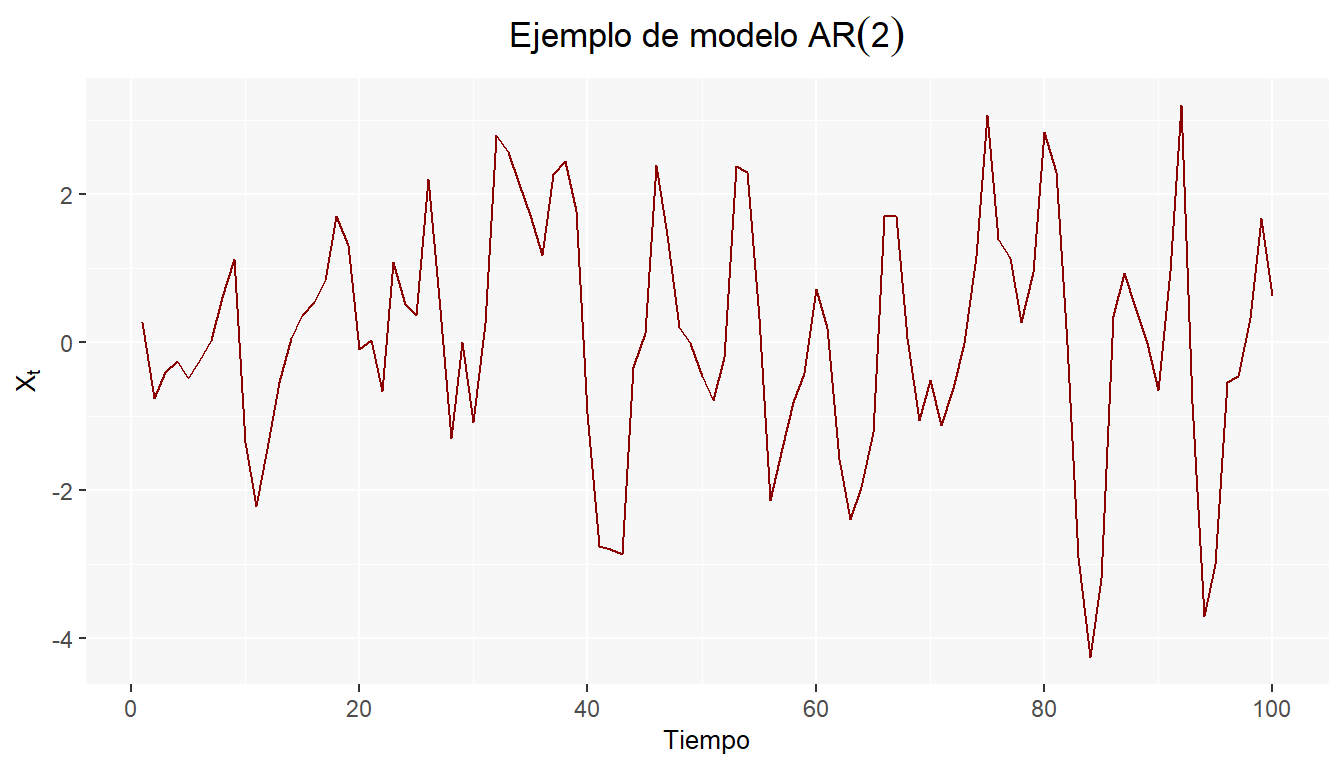
\includegraphics{_main_files/figure-latex/unnamed-chunk-15-1} \end{center}

Y al igual que para el ejemplo del modelo \(AR(1)\), se agregan las gráficas de autocorrelación simple y parcial.

\begin{center}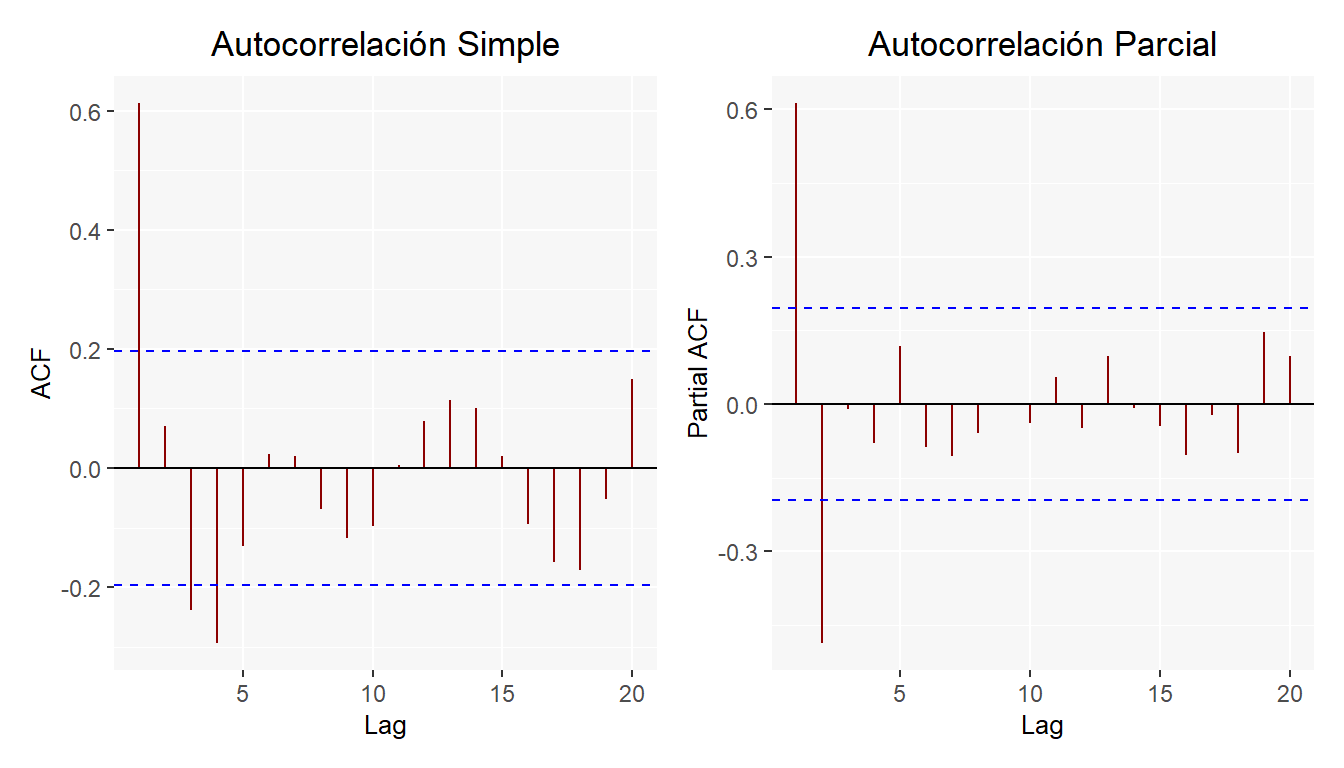
\includegraphics{_main_files/figure-latex/unnamed-chunk-16-1} \end{center}

Algo interesante de tener los procesos en términos de operadores de retardos es que podemos obtener las condiciones de estacionariedad en \(AR\) por las raíces del polinomio que se deriva de esta notación:

\[
\begin{split}
AR(1):& X_t = \phi_1 X_{t-1}+\epsilon_t\\
\implies & (1-\phi_1 B)X_t = \epsilon_t\\
\implies &B = \frac{1}{\phi_1}\implies |\phi_1|<1
\end{split}
\]
\[
\begin{split}
AR(2):& X_t = \phi_1X_{t-1}+\phi_2X_{t-2}+\epsilon_t\\
\implies & (1-\phi_1B-\phi_2B^2)X_t = \epsilon_t
\end{split}
\]

Por lo que las raíces del polinomio \((1-\phi_1B-\phi_2B^2)\) serán \(B^1, B^2 = \frac{\theta_1\pm\sqrt{\theta_1^2+4\theta_2}}{-2\theta_2}\).

Y gracias a todo esto, podemos interpretar que para que los procesos sean estacionarios, se solicita que las raíces estén fuera del círculo unitario, es decir: \(|B^1|>1\) y \(|B^2|>1\).

\hypertarget{maq-proceso-de-medias-muxf3viles}{%
\chapter{\texorpdfstring{\(MA(q)\): Proceso de Medias Móviles}{MA(q): Proceso de Medias Móviles}}\label{maq-proceso-de-medias-muxf3viles}}

Estos modelos se puede decir son determinados por una fuente externa, además de que suponen linealidad. Es decir que el valor actual de la serie \(X_t\) esta influenciado por los valores de la fuente externa.

El modelo de medias móviles de orden \(q\) está dado por:

\[
MA(q): X_t - \mu =\epsilon_t - \theta_1\epsilon_{t-1}-\theta_2\epsilon_{t-2}-...-\theta_q \epsilon_{t-q}
\]

Expresado en términos del operador de retardos

\[
\begin{split}
X_t&=\mu+(1-\theta_1B-\theta_2B^2-...-\theta_qB^q)\epsilon_t\\
&=\mu+\theta_q(B)\epsilon_t
\end{split}
\]
donde \(\epsilon_t\) es un proceso de ruido blanco, \(\theta_1,\theta_2, ..., \theta_q\) son los parámetros del modelo.

Antes de continuar, véase que es posible escribir un modelo \(AR\) con un \(MA\). Supongamos un modelo \(AR(2)\), en el cual se tiene lo siguiente

\[
\begin{array}{ll}
AR(2): X_t = \phi_0+\phi_1X_{t-1}+\phi_2X_{t-2}+\epsilon_t\\
\implies \phi(B)X_t = (1-\phi_1B^1-\phi_2B^2)X_t = \phi_0+\epsilon\\
\therefore X_t = \frac{\phi_0}{\phi(B)}+\frac{\epsilon_t}{\phi(B)} = \mu+(1-\psi_1B^1-\psi_2B^2-\cdots)\epsilon_t
\end{array}
\]

Sin olvidar que las condiciones de estacionalidad para un proceso \(AR(1)\) y \(AR(2)\) son \(|\phi_1|<1\) y \(|1-\phi_1-\phi_2|>0\) respectivamente\footnote{Una pregunta interesante es: ¿Se puede escribir un proceso \(MA\) como un proceso \(AR\)? La respuesta es sí. A esto se le conoce como \textbf{invertibilidad} y al igual que la estacionariedad, esta sucede bajo algunas condiciones. Para más información puede consultarse \citet{cryer2008time}.}.

\hypertarget{proceso-de-medias-muxf3viles-de-orden-1-ma1}{%
\section{\texorpdfstring{Proceso de Medias Móviles de orden 1: \(MA(1)\)}{Proceso de Medias Móviles de orden 1: MA(1)}}\label{proceso-de-medias-muxf3viles-de-orden-1-ma1}}

Este modelo determina el valor de \(X_t\) en función de la innovación actual y su primer retardo, es decir:

\[
\begin{split}
& X_t=\theta_0-\theta_1\epsilon_{t-1}-\epsilon_t = \mu-\theta_1\epsilon_{t-1}-\epsilon_t \\
\implies &X_t=\mu-(1+\theta_1 B)\epsilon_{t}
\end{split}
\]
donde \(\epsilon_t\) es un proceso de ruido blanco y \(\theta\) es el parámetro. Además, véase que

\[
\mathbb{E}(X_t) = \mu-\theta_1\mathbb{E}(\epsilon_{t-1})-\mathbb{E}(\epsilon_{t}) = \mu
\]

Por lo que este proceso ya es estacionario en su media. Sólo resta estudiar el caso para la covarianza. Asumiendo estacionariedad débil, se tiene lo siguiente

\[
\begin{split}
\gamma_0 &= \mathbb{E}\left[(X_{t}-\mathbb{E}(X_{t}))^2\right]=\mathbb{E}\left[(\mu-\theta_1\epsilon_{t-1}-\epsilon_t-\mu)^2\right]\\
& = \mathbb{E}\left[\theta_1^2\epsilon_{t-1}^2+2\theta_1\epsilon_{t-1}\epsilon_{t}+\epsilon_t^2\right]\\
& = \theta_1^2\sigma^2+\sigma^2\\
& =(1+\theta_1^2)\sigma^2\\
\\
\gamma_1 &= \mathbb{E}\left[(X_{t}-\mathbb{E}(X_{t}))(X_{t-1}-\mathbb{E}(X_{t-1}))\right]\\
& =\mathbb{E}\left[(-\epsilon_t-\theta_1\epsilon_{t-1})(-\epsilon_{t-1}-\theta_1\epsilon_{t-2})\right]\\
& = \mathbb{E}\left[\epsilon_t\epsilon_{t-1}+\theta_1\epsilon_t\epsilon_{t-2}+\theta_1\epsilon_{t-1}^2+\theta_1^2\epsilon_{t-1}\epsilon_{t-2}\right]\\
& =\theta_1\mathbb{E}\left[\epsilon_{t-1}^2\right]\\
&= \theta_1\sigma^2\\
\\
\gamma_2 &= \mathbb{E}\left[(X_{t}-\mathbb{E}(X_{t}))(X_{t-2}-\mathbb{E}(X_{t-2}))\right] = 0\\
\vdots
\end{split}
\]

Entonces la \textbf{función de autocovarianza} de un modelo \(MA(1)\) es:

\[
\gamma_k = \left\{
\begin{array}{lr}
(1+\theta^2)\sigma^2 &   \mbox{ si } k=0\\
\theta_1 \sigma^2 & \mbox{ si } k=1\\
0 &    \mbox{ si } k>1\\
\end{array}
\right.
\]

Y la correspondiente \textbf{función de autocorrelación} de un modelo \(MA(1)\) es:

\[
\rho_k = \frac{\gamma_k}{\gamma_0} = \left\{
\begin{array}{lr}
1 &  \mbox{ si } k=0\\
\frac{\theta_1}{1+\theta_1^2} &  \mbox{ si } k=1\\
0 & \mbox{ si } k>1\\
\end{array}
\right.
\]
A continuación se muestran los resultados para un modelo \(AR(1)\) de la siguiente forma \(X_t=0.45\epsilon_{t-1}\)

\begin{center}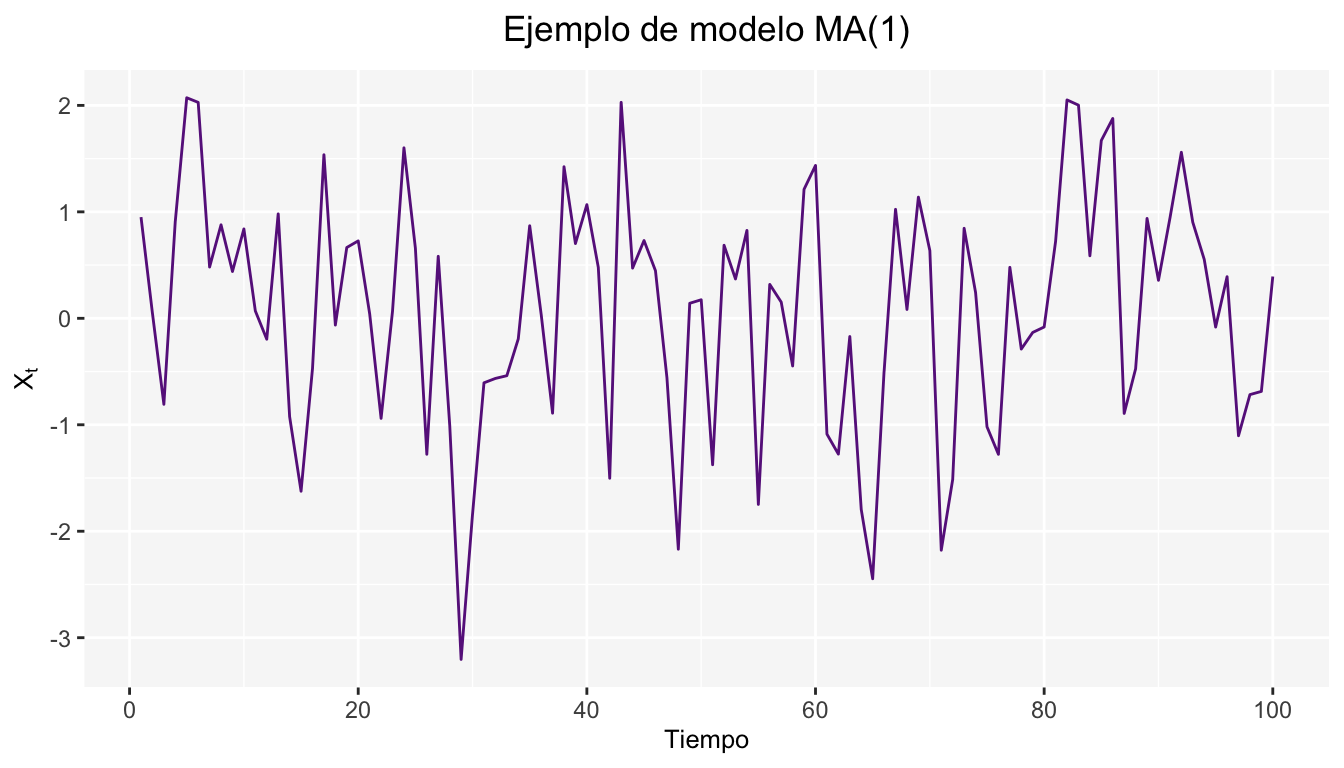
\includegraphics{_main_files/figure-latex/unnamed-chunk-17-1} \end{center}

Además de las gráficas de Autocorrelación simple y parcial.

\begin{center}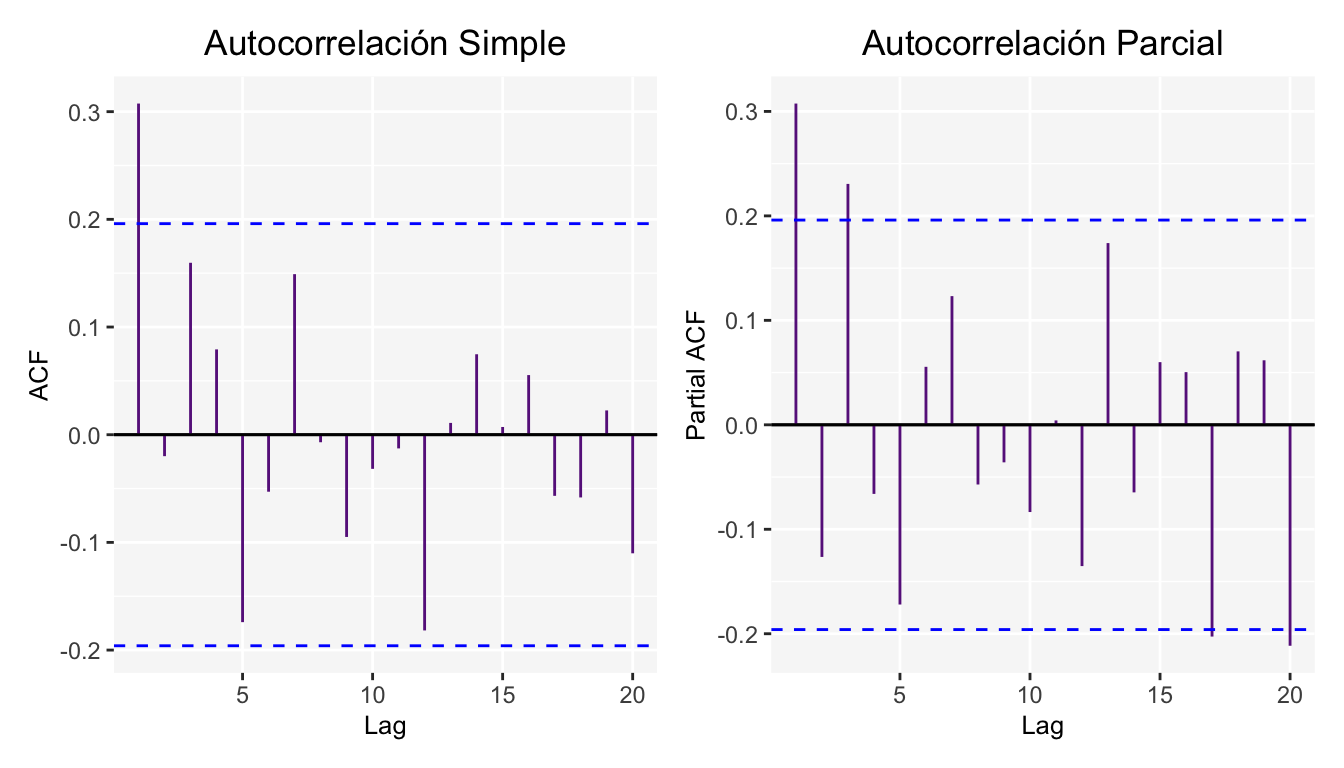
\includegraphics{_main_files/figure-latex/unnamed-chunk-18-1} \end{center}

\hypertarget{proceso-de-medias-muxf3viles-de-orden-2-ma2}{%
\section{\texorpdfstring{Proceso de Medias Móviles de orden 2: \(MA(2)\)}{Proceso de Medias Móviles de orden 2: MA(2)}}\label{proceso-de-medias-muxf3viles-de-orden-2-ma2}}

Este modelo esta determinado por:

\[
\begin{split}
MA(2): X_t & = \theta_0-\epsilon_t-\theta_1\epsilon_{t-1}-\theta_2\epsilon_{t-2}\\
X_t & = \theta_0-(1+\theta_1 B+\theta_2B^2)\epsilon_{t}
\end{split}
\]

donde \(\epsilon_t\) es un proceso de ruido blanco y \(\theta_1,\theta_2\) son los parámetros del modelo. Asumiendo estacionariedad débil, es fácil comprobar que \(\mathbb{E}(X_t) = \theta_0\). Respecto a la covarianza se tiene lo siguiente

\[
\begin{split}
\gamma_0 & = \mathbb{E}\left[(X_{t}-\mathbb{E}(X_{t}))^2\right]=\mathbb{E}\left[(-\epsilon_t-\theta_1\epsilon_{t-1}-\theta_2\epsilon_{t-2})^2\right]\\
& = \mathbb{E}\left[\epsilon_t^2\right]+\theta_1^2\mathbb{E}\left[\epsilon_{t-1}\right]^2+\theta_2^2\mathbb{E}\left[\epsilon_{t-2}\right]^2\\
& = \left(1+\theta_1^2+\theta_2^2\right)\sigma^2\\
\\
\gamma_1 & = \mathbb{E}\left[(X_{t}-\mathbb{E}(X_{t}))(X_{t-1}-\mathbb{E}(X_{t-1}))\right]\\
& = \mathbb{E}\left[(-\epsilon_t-\theta_1\epsilon_{t-1}-\theta_2\epsilon_{t-2})(-\epsilon_{t-1}-\theta_1\epsilon_{t-2}-\theta_2\epsilon_{t-3})\right]\\
& = \mathbb{E}\left[\theta_1\epsilon_{t-1}^2+\theta_1\theta_2\epsilon_{t-2}^2\right]\\
& = \theta_1\left(1+\theta_2\right)\sigma^2\\
\\
\gamma_2 & = \mathbb{E}\left[(X_{t}-\mathbb{E}(X_{t}))(X_{t-2}-\mathbb{E}(X_{t-2}))\right]\\
& = \mathbb{E}\left[(-\epsilon_t-\theta_1\epsilon_{t-1}-\theta_2\epsilon_{t-2})(-\epsilon_{t-2}-\theta_1\epsilon_{t-3}-\theta_2\epsilon_{t-4})\right]\\
& = \theta_2\mathbb{E}\left[\epsilon_{t-2}^2\right]\\
& = \theta_2\sigma^2
\end{split}
\]

Entonces la \textbf{función de autocovarianza} de un modelo \(MA(2)\) es:

\[
\gamma_k = \left\{
\begin{array}{lr}
\left(1+\theta_1^2+\theta_2^2\right)\sigma^2 & \mbox{ si } k=0\\
\theta_1(1+\theta_2) \sigma^2 & \mbox{ si }\ k=1\\
\theta_2 \sigma^2 & \mbox{ si } k=2\\
0 & \mbox{ si } k>2\\
\end{array}
\right.
\]

Y la correspondiente \textbf{función de autocorrelación} de un modelo \(MA(2)\) es:

\[
\rho_k = \left\{
\begin{array}{lr}
1 &  \mbox{ si } k=0\\
\frac{\theta_1+(1+\theta_2)}{1+\theta_1^2+\theta_2^2}&  \mbox{ si } k=1\\
\frac{\theta_2}{1+\theta_1^2+\theta_2^2}&  \mbox{ si } k=2\\
0 &  \mbox{ si }  k>2\\
\end{array}
\right.
\]

\hypertarget{armapq-proceso-autoregresivo-de-medias-muxf3viles}{%
\chapter{\texorpdfstring{\(ARMA(p,q)\): Proceso Autoregresivo de Medias Móviles}{ARMA(p,q): Proceso Autoregresivo de Medias Móviles}}\label{armapq-proceso-autoregresivo-de-medias-muxf3viles}}

Es muy probable que una serie de tiempo \(X_t\), tenga características de un proceso \(AR\) y de un proceso \(MA\) al mismo tiempo, por lo que será un proceso \(ARMA\). Así, \(X_t\) sigue un proceso \(ARMA(p,q)\), y en este proceso habrá \(p\) términos autoregresivos y \(q\) términos de media móvil. Este se verá de la siguiente forma:

\[
X_t=c+ \phi_1X_{t-1}+...+\phi_pX_{t-p}+-\theta_1\epsilon_{t-1}-\theta_2\epsilon_{t-2}-...-\theta_q\epsilon_{t-q}+\epsilon_t
\]

donde \(\epsilon_t\) es un proceso de ruido blanco, y \(\phi_1,...,\phi_p,\theta_1,...,\theta_q\) son los parámetros del modelo.

Para un proceso \(ARMA(p,q)\) una condición de estacionariedad es la misma que para un proceso \(AR(p)\), y una condición de invertivilidad es la misma que para el proceso \(MA(q)\).

El modelo \(ARMA(p,q)\) se puede escribir en términos de los operadores de retardo de la siguiente manera.

Sea \(c = 0\).

\[
\begin{array}{c}
(1-\phi_1B-\phi_2B^2-...-\phi_pB^p)X_t=(1-\theta_1B-\theta_2B^2-...-\theta_qB^q)\epsilon_t\\
\implies \phi_p(B)X_t=\theta_q(B)\epsilon_t
\end{array}
\]

Donde
+ \(\phi_p(B)\) es el polinomio autoregresivo
+ \(\theta_q(B)\) es el polinomio de medias móviles.

Hay que observar lo siguiente:

\[
\begin{array}{lr}
X_t = \frac{\theta_q(B)}{\phi_p(B)}\epsilon_t & \longleftarrow MA(\infty)\\
\epsilon_t = \frac{\phi_1(B)}{\theta_q(B)}X_t & \longleftarrow AR(\infty)
\end{array}
\]

\begin{itemize}
\tightlist
\item
  Los modelos \(ARMA(p,q)\) siempre compartirán las características de los modelos \(AR(p)\) y \(MA(q)\), ya que contiene ambas estructuras a la vez.
\item
  El modelo \(ARMA(p,q)\) tiene media cero y varianza constante y finita además de que la función de autocorrelación es infinita y decrece rápidamente hacia cero.\\
\item
  Un proceso \(ARMA(p,q)\) es \textbf{estacionario} si y sólo si el modulo de las raíces del polinomio \(\phi_p(B)\) está fuera del círculo unitario.
\item
  Un proceso \(ARMA(p,q)\) es \textbf{invertible} si y sólo si el modulo de las raíces del polinomio \(\theta_q(B)\) está fuera del círculo unitario.
\end{itemize}

\textbf{Ejemplo}

Sea \(Y_t: ARMA(2,1)\) con \(\epsilon_t\sim N(0,1)\) tal que \(Y_t = 1.5Y_{t-1}-0.9Y_{t-2}-0.4\epsilon_{t-1}+\epsilon_t\).

Sabemos que es invertible por que \(|\theta| = |-0,4|<1\) y es estacionario por lo siguiente:

\[
\begin{split}
&\phi_2(B) = (1-1.5B+0.9B^2)\\
\implies & B_1, B_2 = \frac{1.5\pm\sqrt{1.5^2-4(0.9)}}{2(0.9)} = 0.83\pm0.645\\
\implies & |B| = \sqrt{0.83^2+0.65^2} = 1.05423 > 1
\end{split}
\]

\hypertarget{arma11}{%
\section{\texorpdfstring{\(ARMA(1,1)\)}{ARMA(1,1)}}\label{arma11}}

En un modelo \(ARMA(1,1)\) la serie de tiempo \(X_t\) se determina en función de su pasado hasta el primer retardo, la innovación actual y el pasado de la innovación hasta el primer retardo.

\[
X_t=c+ \phi_1X_{t-1}+\epsilon_t-\theta_1\epsilon_{t-1}
\]

donde \(\epsilon_t\) es un proceso de ruido blanco, y \(\phi_1\) y \(\theta_1\) son los parámetros del modelo. Ahora se verán las características de un proceso \(ARMA(1,1)\) estacionario.

\hypertarget{media}{%
\subsection{Media}\label{media}}

\[
\begin{array}{l}
\mathbb{E}(X_t)=\mathbb{E}(c+ \phi_1X_{t-1}+\epsilon_t-\theta_1\epsilon_{t-1})=c+ \phi_1\mathbb{E}(X_{t-1})\\
\end{array}
\]

Por lo que Suponiendo estacionariedad \(\mathbb{E}(X_t) = \frac{c}{1-\theta_1}\).

\hypertarget{covarianzas}{%
\subsection{Covarianzas}\label{covarianzas}}

\[
\begin{split}
\gamma_0 &=\mathbb{E}\left[(X_t-\mathbb{E}(X_t))^2\right]=\phi_1^2Var(X_{t-1})+\theta_1^2\sigma^2+\sigma^2+\phi_1\theta_1Cov(X_{t-1}, \epsilon_{t-1})\\
\Longleftrightarrow & (1-\phi_1^2)Var(X_t) = \sigma^2(1+\theta_1^2)+\phi_1\theta_1\sigma^2\\
\implies & Var(X_t) = \gamma_0 = \frac{\sigma^2(1+\theta_1^2+2\phi_1\theta_1)}{1-\phi_1^2}
\end{split}
\]
Recordando que \(\mathbb{E}(X_t) = c+ \phi_1\mathbb{E}(X_{t-1}) \implies X_t-\mathbb{E}(X_t) = \phi_1(X_{t-1}-\mathbb{E}(X_{t-1}))+\epsilon_t+\theta\epsilon_{t-1}\)

\[
\begin{split}
\gamma_1 & =\mathbb{E}[(X_t-\mathbb{E}(X_t))(X_{t-1}-\mathbb{E}(X_{t-1}))]\\
& = \mathbb{E}\left[(\phi_1(X_{t-1}-\mathbb{E}(X_{t-1}))+\epsilon_t+\theta_1\epsilon_{t-1})(X_{t-1}-\mathbb{E}(X_{t-1}))\right]\\
& = \mathbb{E}\left[\phi_1(X_{t-1}-\mathbb{E}(X_{t-1}))^2\right] + \mathbb{E}\left[\epsilon_tX_{t-1}\right]-\mathbb{E}\left[\epsilon_t\mathbb{E}(X_{t-1})\right]+\theta_1\mathbb{E}\left[\epsilon_{t-1}X_{t-1}\right]-\theta_1\mathbb{E}[\epsilon_{t-1}\mathbb{E}(X_{t-1})]\\
&= \phi_1\gamma_0+\theta_1\mathbb{E}[\epsilon_{t-1}X_{t-1}]\\
&= \phi_1\gamma_0 + \theta_1\mathbb{E}[\epsilon_{t-1}(c+\phi_1X_{t-2}+\epsilon_{t-1}+\theta_1\epsilon_{t-2})]\\
&= \phi_1\gamma_0 +\theta_1\mathbb{E}\left[c\epsilon_{t-1}+\epsilon_{t-1}\phi_1X_{t-2}+\epsilon_{t-1}^2+\theta_1\epsilon_{t-1}\epsilon_{t-2}\right]\\
&= \phi_1\gamma_0+\theta_1\sigma^2
\end{split}
\]

\[
\begin{split}
\gamma_2 & =\mathbb{E}[(X_t-\mathbb{E}(X_t))(X_{t-2}-\mathbb{E}(X_{t-2}))]\\
& = \mathbb{E}\left[(\phi_1(X_{t-1}-\mathbb{E}(X_{t-1}))+\epsilon_t+\theta_1\epsilon_{t-1})(X_{t-2}-\mathbb{E}(X_{t-2}))\right]\\
& = \mathbb{E}\left[(\phi_1(X_{t-1}-\mathbb{E}(X_{t-1}))(X_{t-2}-\mathbb{E}(X_{t-2}))+\epsilon_t(X_{t-2}-\mathbb{E}(X_{t-2}))+\theta_1\epsilon_{t-1}(X_{t-2}-\mathbb{E}(X_{t-2}))\right]\\
&= \mathbb{E}[\phi_1(X_{t-1}X_{t-2}-X_{t-1}\mathbb{E}(X_{t-2})-X_{t-2}\mathbb{E}(X_{t-1})+\mathbb{E}(X_{t-1})\mathbb{E}(X_{t-2}))\\
& \ \ \ \ \ + \epsilon_tX_{t-2}-\epsilon_t\mathbb{E}(X_{t-2})+\theta_1\epsilon_{t-1}X_{t-2}-\theta_1\epsilon_{t-1}\mathbb{E}(X_{t-2})]\\
&= \phi_1\gamma_1
\end{split}
\]

Entonces la \textbf{función de autocovarianza} de un proceso \(ARMA(1,1)\) es:

\[  
\gamma_{k} =
\begin{cases}
\frac{\sigma^2(1+\theta_1^2+2\phi_1\theta_1)}{1-\phi_1^2} & k=0\\
\phi_1\gamma_0+\theta_1\sigma^2 & k=1\\
\phi_1\gamma_{k-1} & k>1
\end{cases}       
\]
Y la \textbf{función de autocorrelación} de un proceso \(ARMA(1,1)\) es:

\[ 
\rho_{k} =
\begin{cases}
1 & k=0\\
\frac{\phi_1\gamma_0+\theta_1\sigma_2}{\gamma_0}=\phi_1-\frac{\theta_1\sigma^2}{\gamma_0} & k=1\\
\frac{\phi_1\gamma_{k-1}}{\gamma_0} = \phi_1\rho_{k-1} & k>1
\end{cases}       
\]
A continuación se muestran los resultados para un modelo \(ARMA(1,1)\) de la siguiente forma \(X_t=0.65X_{t-1}+.30\epsilon_{t-1}\)

\begin{center}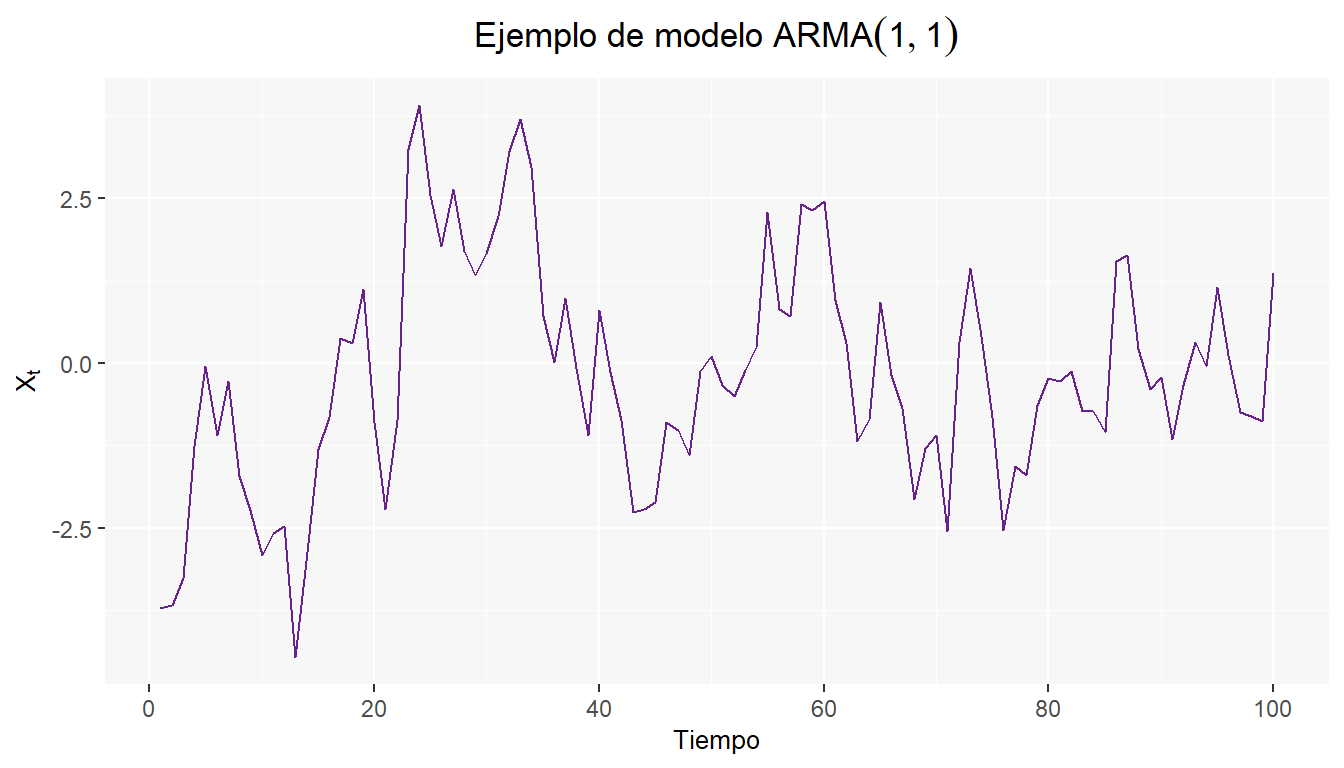
\includegraphics{_main_files/figure-latex/unnamed-chunk-19-1} \end{center}

Además de las gráficas de Autocorrelación simple y parcial.

\begin{center}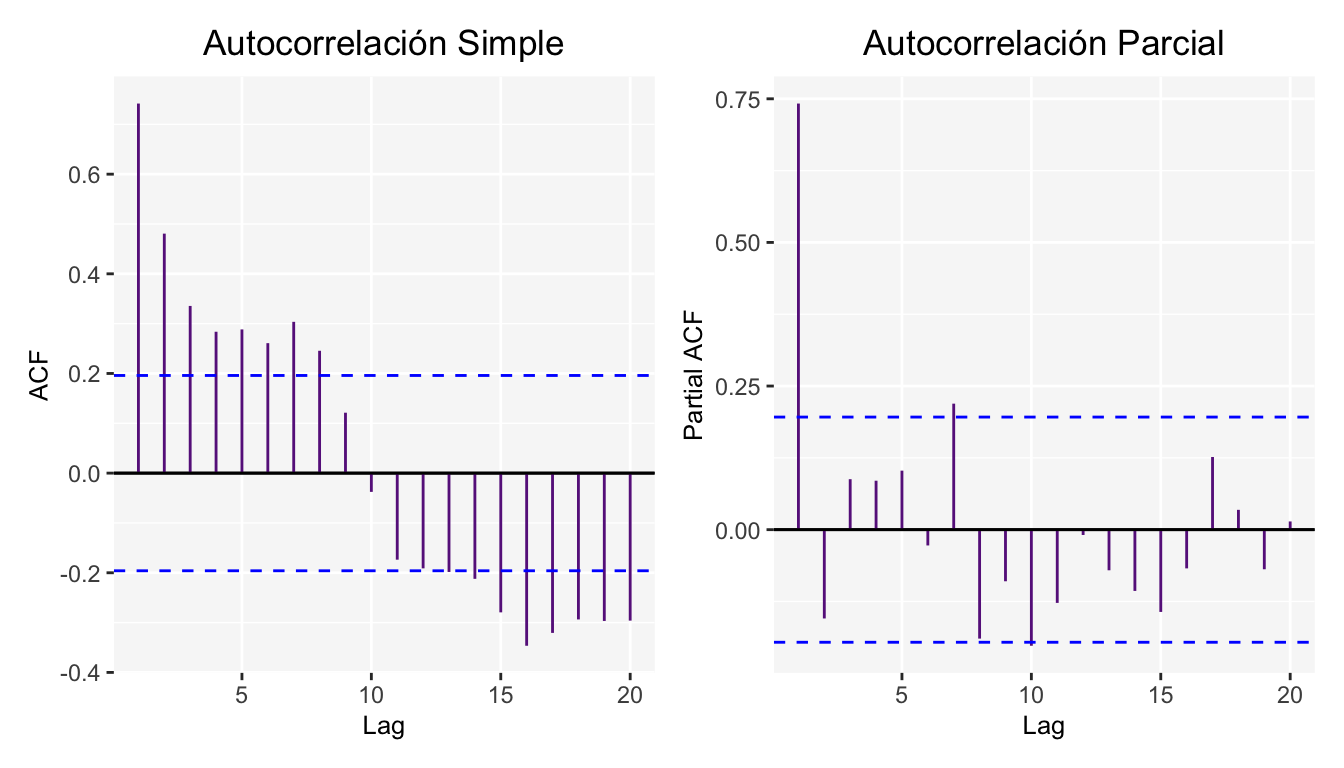
\includegraphics{_main_files/figure-latex/unnamed-chunk-20-1} \end{center}

\hypertarget{part-procesos-lineales-no-estacionarios}{%
\part{Procesos lineales no estacionarios}\label{part-procesos-lineales-no-estacionarios}}

\hypertarget{arimapdq-proceso-autoregresivo-integrado-y-de-medias-muxf3viles}{%
\chapter{\texorpdfstring{\(ARIMA(p,d,q)\): Proceso Autoregresivo Integrado y de Medias Móviles}{ARIMA(p,d,q): Proceso Autoregresivo Integrado y de Medias Móviles}}\label{arimapdq-proceso-autoregresivo-integrado-y-de-medias-muxf3viles}}

Los modelos de series de tiempo \(AR\), \(MA\) y \(ARMA\) se basan en el supuesto de estacionariedad del proceso, es decir, la media, la varianza y las covarianzas son constantes en el tiempo. Sin embrago, muchas series de tiempo relacionadas con aplicaciones reales no son estacionarias, ya sea porque cambian de nivel en el tiempo (existe tendencia) o la varianza no es constante en el tiempo, a este tipo de procesos se les conoce como \textbf{procesos integrados}.

Para trabajar con estas series de tiempo lo que se hace es calcular las diferencias de la serie de tiempo \(d\) veces para hacerla estacionaria y posteriormente aplicar a la serie diferenciada un modelo \(ARMA(p,q)\), en este caso se diría que la serie original es un proceso \(ARIMA(p,d,q)\), donde \(p\) es el número de términos autoregresivos, \(d\) el número de veces que la serie debe ser diferenciada para hacerla estacionaria y \(q\) el número de términos de la media móvil.

La expresión algebraica del proceso \(ARIMA(p,d,q)\) es:

\[
X_t^d=c+\phi_1X_{t-1}^d+...+\phi_pX_{t-p}^d-\theta_1\epsilon_{t-1}^d-\theta_2\epsilon_{t-2}^d-...-\theta_q\epsilon_{t-q}^d+\epsilon_t^d
\]

donde \(X_t^d\) es la serie de las diferencias de orden \(d\), \(\epsilon_t^d\) es un proceso de ruido blanco, y \(\phi_1,...,\phi_p,\theta_1,...,\theta_q\) son los parámetros del modelo.

El modelo \(ARIMA(p,d,q)\) se puede escribir en términos de los operadores de retardo de la siguiente manera:

\[
\begin{array}{c}
(1-\phi_1B-\phi_2B^2-...-\phi_pB^p)X_t^d=c+(1-\theta_1B-\theta_2B^2-...-\theta_qB^q)\epsilon_t^d\\
\phi_p(B)(1-B)^dX_t=c+\theta_q(B)\epsilon_t^d
\end{array}
\]
Los modelos integrados se usan para reducir la \textbf{NO} estacionariedad de la serie al usar las diferencias y en la mayoría de las aplicaciones \(d=1\) y hasta \(d=2\) es suficiente para volver la serie estacionaria, pero en algunas ocasiones, aplicar transformaciones a los datos tienen mejor resultado para lograr la estacionariedad en comparación con las diferencias. Por ejemplo, en las series de tiempo económicas, la variabilidad aumenta cuando el nivel promedio del proceso aumenta. Sin embargo el porcentaje de cambio en las observaciones es relativamente independiente del nivel, entonces aplicar una transformación logarítmica puede ser más eficiente para lograr la estacionariedad de la serie.

\textbf{Ejemplo}

Se tiene el siguiente modelo: \(X_t = \mu_t +Z_t\) donde \(\mu_t = \beta_0+\beta_1t\) y \(Z_t\) es un proceso estacionario.

\[
\begin{split}
X_t -X_{t-1} &= \mu_t+Z_t-\mu_{t-1}-Z_{t-1}\\
& = \beta_0+\beta_1t+Z_t-\beta_0-\beta_1(t-1)-Z_{t-1}\\
& = \beta_1+Z_t-Z_{t-1}
\end{split}
\]

El cual ya no depende de \(t\).

A continuación se muestran los resultados para un modelo \(ARIMA(2,1,1)\) de la siguiente forma \(X_t=0.85X_{t-1}-0.45X_{t-2}+.30\epsilon_{t-1}\)

\begin{center}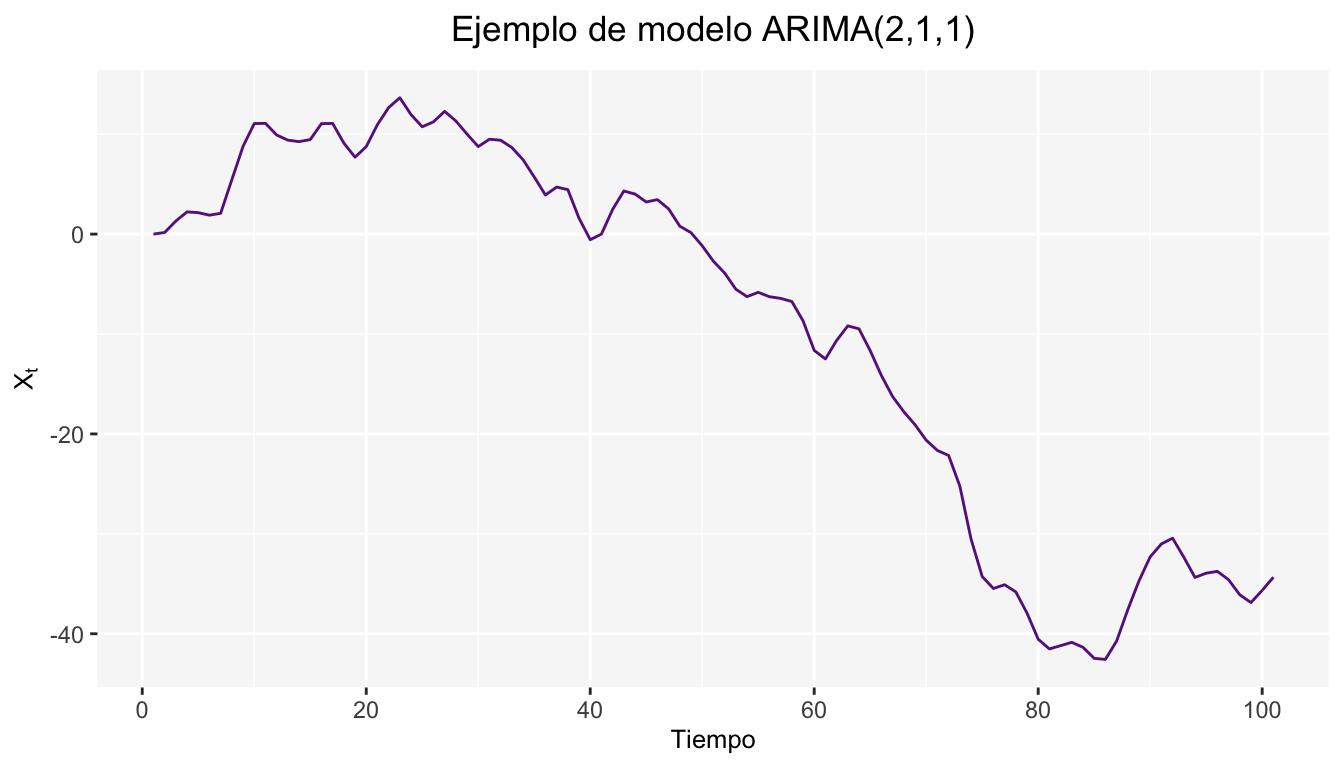
\includegraphics{_main_files/figure-latex/unnamed-chunk-21-1} \end{center}

Además de las gráficas de Autocorrelación simple y parcial.

\begin{center}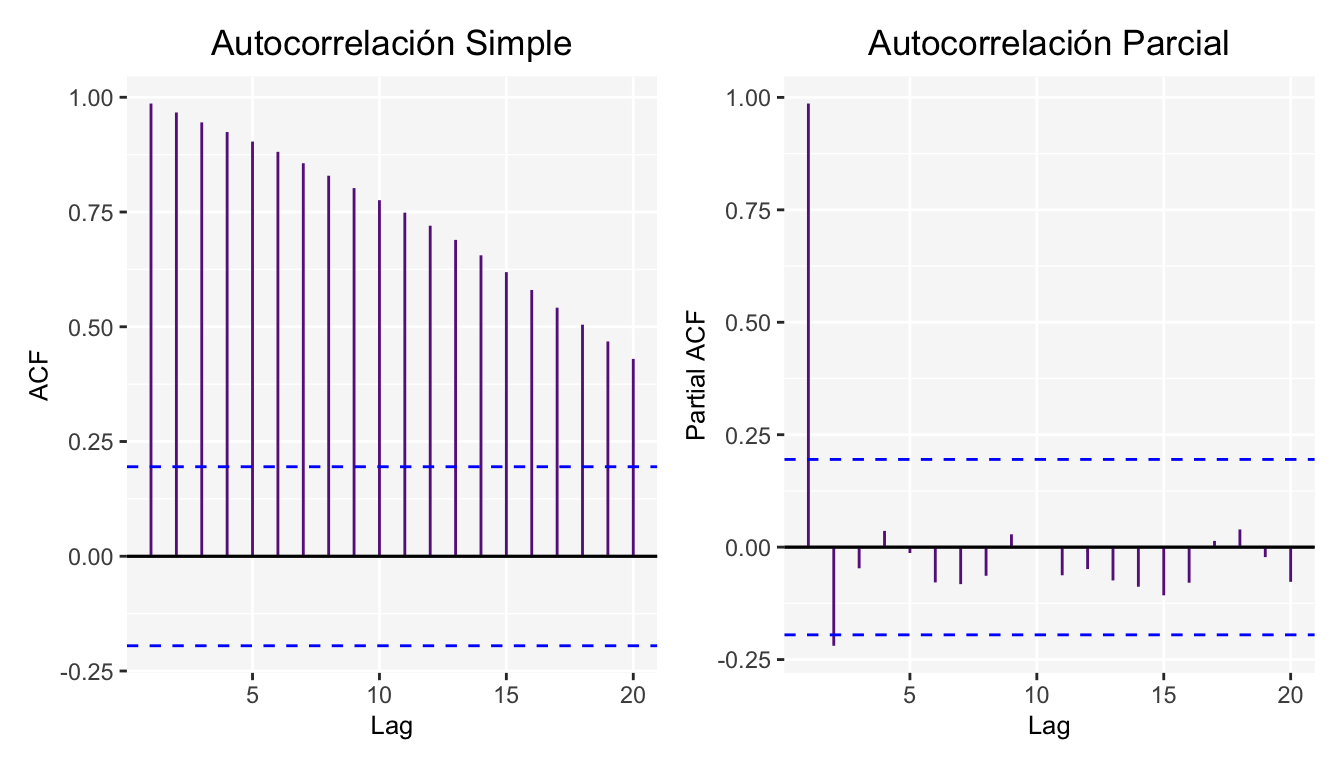
\includegraphics{_main_files/figure-latex/unnamed-chunk-22-1} \end{center}

A continuación se muestran los resultados para un modelo \(ARIMA(2,2,1)\) de la siguiente forma \(X_t=0.85X_{t-1}-0.45X_{t-2}+.30\epsilon_{t-1}\)

\begin{center}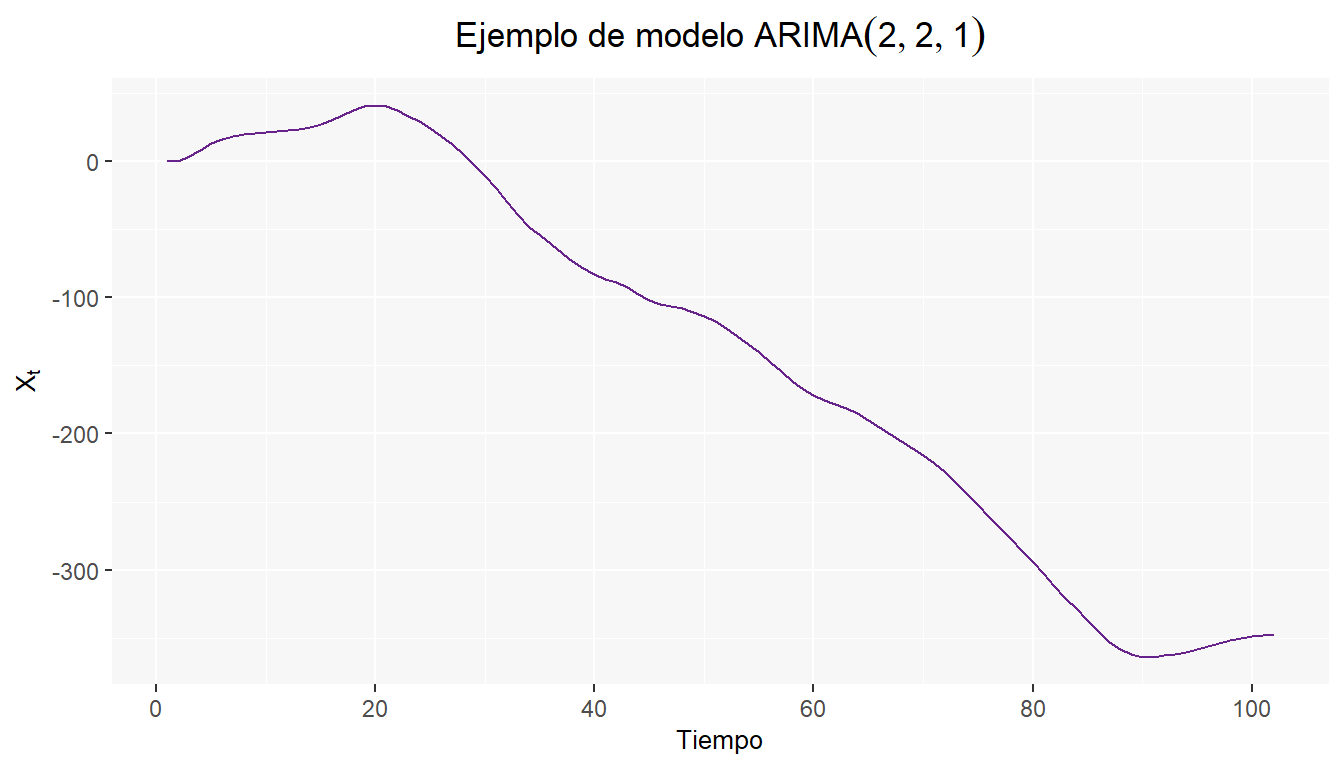
\includegraphics{_main_files/figure-latex/unnamed-chunk-23-1} \end{center}

Además de las gráficas de Autocorrelación simple y parcial.

\begin{center}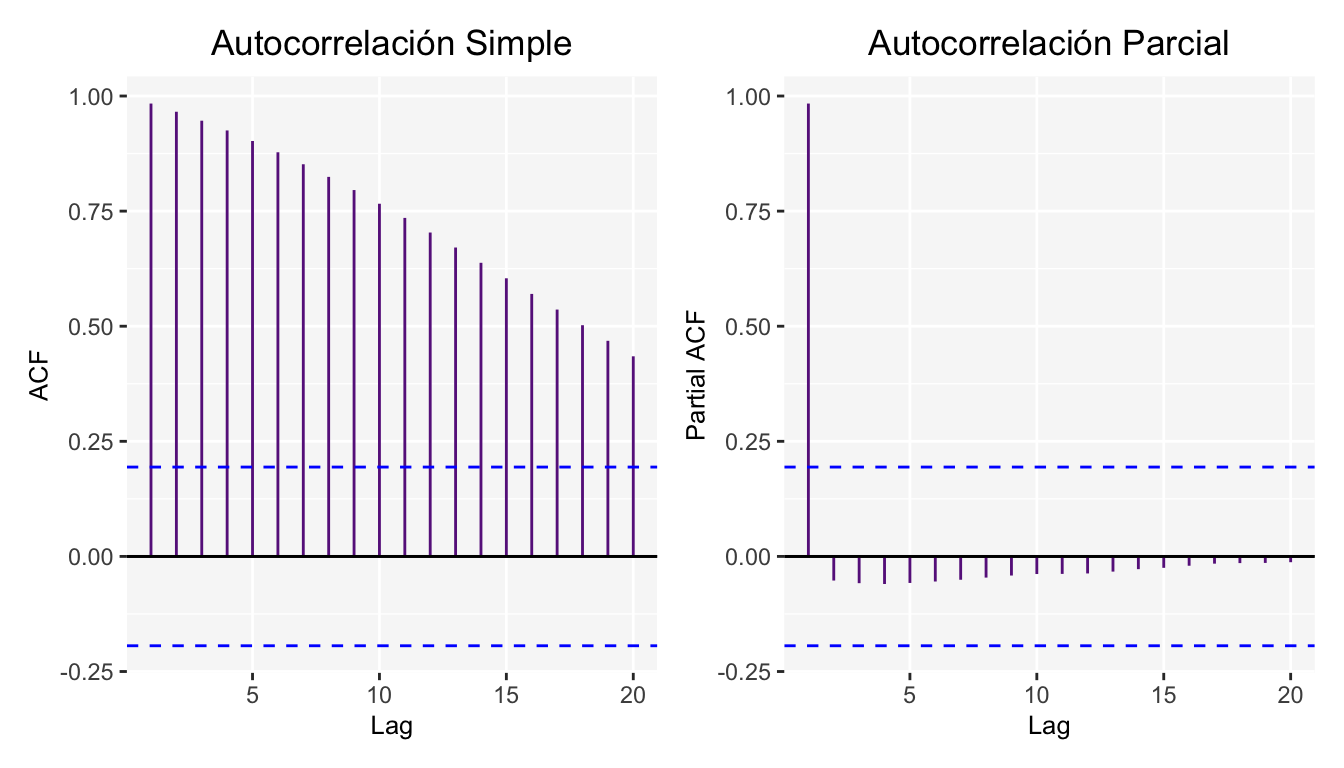
\includegraphics{_main_files/figure-latex/unnamed-chunk-24-1} \end{center}

¿Qué se puede decir del efecto que tiene el parámetro \(d\) al comparar las gráficas de ambas series?

\hypertarget{imadq-proceso-integrado-y-de-media-muxf3vil}{%
\chapter{\texorpdfstring{\(IMA(d,q)\): Proceso Integrado y de Media Móvil}{IMA(d,q): Proceso Integrado y de Media Móvil}}\label{imadq-proceso-integrado-y-de-media-muxf3vil}}

Este proceso es un caso particular del proceso \(ARIMA(p,d,q)\) cuando \(p=0\). Se calculan las diferencias de la serie de tiempo \(d\) veces para convertir la serie en estacionaria y luego se aplica un modelo \(MA(q)\).

Por ejemplo:

Sea \(Z_1, Z_2, Z_3, Z_4, Z_5\) la serie de tiempo original. Entonces la serie diferenciada de orden uno será:

\[
\begin{array}{c}
Y_1=Z_2-Z_1\\
Y_2=Z_3-Z_2\\
Y_3=Z_4-Z_3\\
Y_4=Z_5-Z_4
\end{array}
\]

Y la serie diferenciada de orden dos será:

\[
\begin{split}
X_1=Y_2+Y_1=Z_3-Z_2+Z_2-Z_1=Z_3-Z_1\\
X_2=Y_3+Y_2=Z_4-Z_2\\
X_3=Y_4+Y_3=Z_5-Z_3
\end{split}
\]
Por lo tanto al hacer diferencia de orden 2 a la serie de tiempo original \(Z_t\), se obtiene una serie de tiempo \(X_1, X_2, X_3\) que ya es estacionaria y a esta se la aplicaría un modelo de medias móviles \(MA(q)\), por ejemplo si \(q=1\) se ajustaría un modelo \(X_t=X_{t-1}+\epsilon_t\), donde \(\epsilon_t\) es ruido blanco.

A continuación se modelan los datos de un modelo \(MA(3)\) de la siguiente forma \(X_t=0.80\epsilon_{t-1}+0.20\epsilon_{t-2}+0.50\epsilon_{t-3}\)

\begin{center}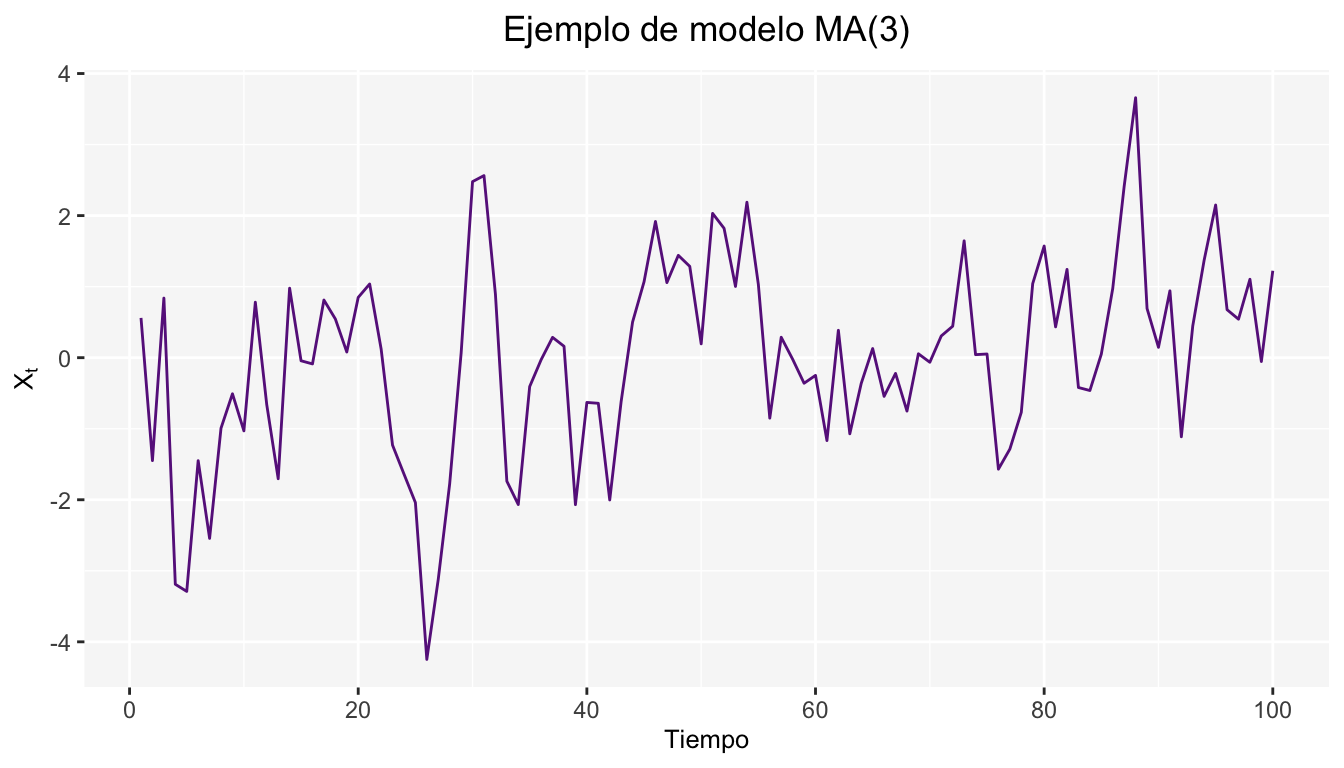
\includegraphics{_main_files/figure-latex/unnamed-chunk-25-1} \end{center}

Además de las gráficas de Autocorrelación simple y parcial.

\begin{center}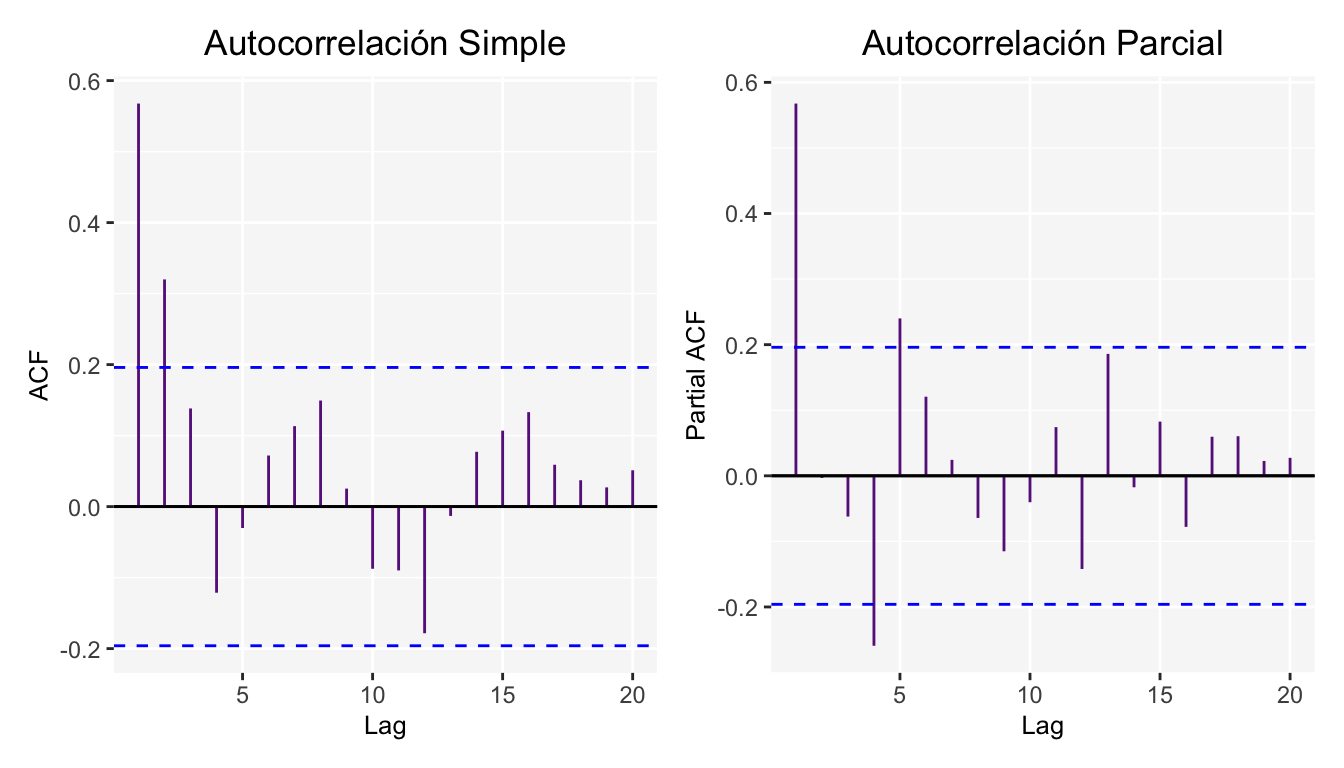
\includegraphics{_main_files/figure-latex/unnamed-chunk-26-1} \end{center}

Ahora veamos como queda la serie si le incluimos un proceso integrado (una diferencia) de orden 1.

\begin{center}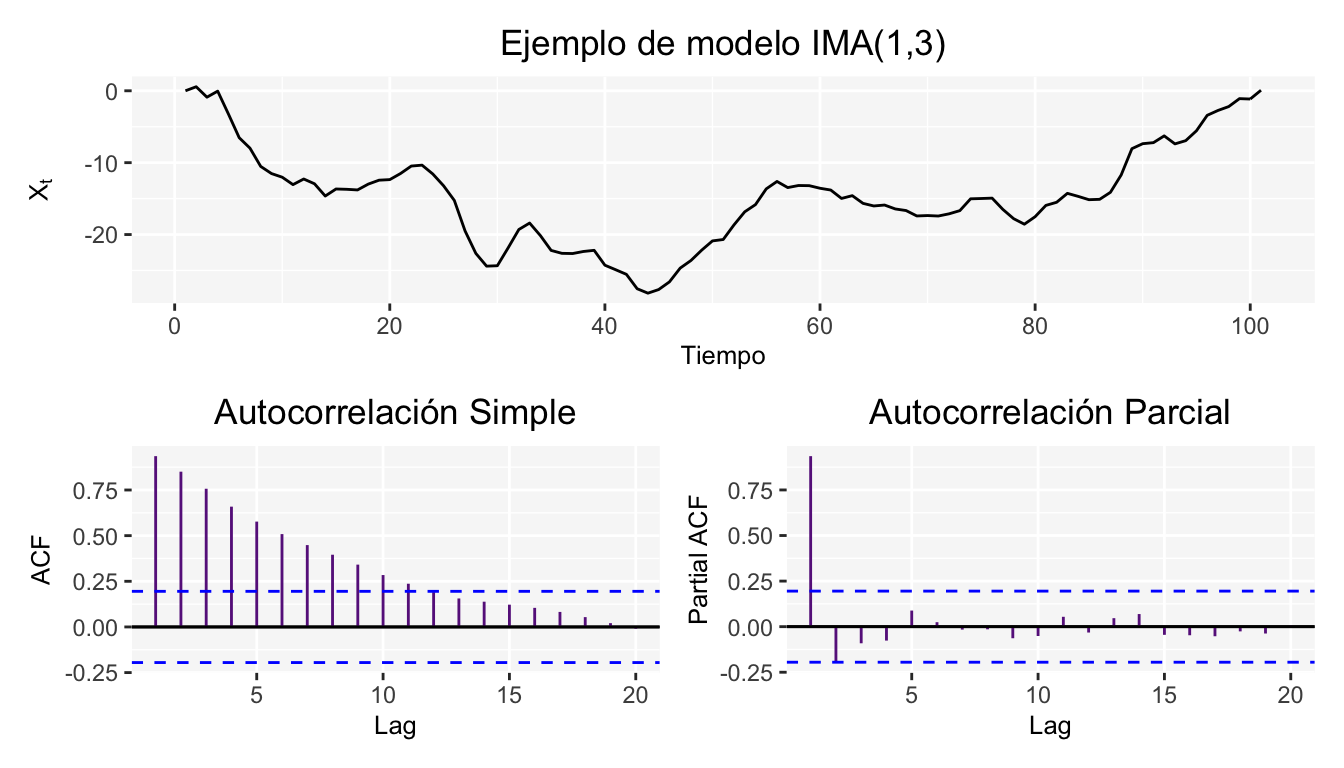
\includegraphics{_main_files/figure-latex/unnamed-chunk-27-1} \end{center}

Haga la prueba aumentando el orden de las diferencias, ¿cuál es el efecto en la serie de tiempo?

\hypertarget{part-otras-consideraciones}{%
\part{Otras consideraciones}\label{part-otras-consideraciones}}

\hypertarget{predictores-lineales}{%
\chapter{Predictores Lineales}\label{predictores-lineales}}

Sea \(X_t\) un proceso estacionario. Se desea predecir \(X_{n+1}\) en una función lineal de lo observado hasta el tiempo \(n\) es decir con \({X_1,X_2,...,X_n}\).
Entonces lo que buscamos es encontrar los coeficientes \(a_i\) con \(i=1,...,n\) tales que

\[
\hat{X}_{n+1}=a_1X_n+a_2X_{n-1}+...+a_nX_1
\]

Utilizando las varianzas y covarianzas entre los elementos de la serie de tiempo se obtiene que una estimación de las \(a_i's\) son las que den solución al siguiente sistema:

\[
\begin{bmatrix}
    Cov(X_1,X_1)       & Cov(X_1,X_2)  & Cov(X_1,X_3) & \dots & Cov(X_1,X_n)  \\
    Cov(X_2,X_1)        & Cov(X_2,X_2)  & Cov(X_2,X_3)  & \dots &Cov(X_2,X_n)  \\
      \vdots & \vdots & \vdots & \ddots & \vdots \\ \\
    Cov(X_n,X_1)        & Cov(X_n,X_2)  & Cov(X_n,X_3)  & \dots & Cov(X_n,X_n) 
\end{bmatrix}
\begin{bmatrix}
a_1\\
a_2\\
\vdots\\
a_n\\
\end{bmatrix}
= \\
\begin{bmatrix}
Cov(X_{n+1},X_n)  \\
Cov(X_{n+1},X_{n-1})  \\
    \vdots\\
Cov(X_{n+1},X_1)  \\
\end{bmatrix}
\]

\[
\Gamma\underline{a} = \begin{bmatrix}
    \gamma_0      & \gamma_1  & \gamma_2 & \dots & \gamma_{n-1}  \\
   \gamma_1       & \gamma_0  & \gamma_1  & \dots &\gamma_{n-2}  \\
      \vdots & \vdots & \vdots & \ddots & \vdots \\ \\
    \gamma_{n-1}       & \gamma_{n-2}  & \gamma_{n-3}  & \dots & \gamma_0 
\end{bmatrix}
\begin{bmatrix}
a_1\\
a_2\\
\vdots\\
a_n\\
\end{bmatrix}
=
\begin{bmatrix}
\gamma_1  \\
\gamma_2  \\
    \vdots\\
\gamma_{n}\\
\end{bmatrix} = \gamma
\]
En general si deseamos predecir \(X_{n+h}\) dado \({X_1,X_2,...,X_n}\), el predictor lineal será

\[
\hat{X}_{n+h}=a_1X_n+a_2X_{n-1}+...+a_nX_1
\]

En donde el mejor predictor lineal serán los \(a_1,a_2,...,a_n\) tales que

\[
\begin{bmatrix}
    \gamma_0      & \gamma_1  & \gamma_2 & \dots & \gamma_{n-1}  \\
   \gamma_1       & \gamma_0  & \gamma_1  & \dots &\gamma_{n-2}  \\
      \vdots & \vdots & \vdots & \ddots & \vdots \\ \\
    \gamma_{n-1}       & \gamma_{n-2}  & \gamma_{n-3}  & \dots & \gamma_0 
\end{bmatrix}
\begin{bmatrix}
a_1\\
a_2\\
\vdots\\
a_n\\
\end{bmatrix}
=
\begin{bmatrix}
\gamma_h  \\
\gamma_{h+1}  \\
    \vdots\\
\gamma_{h+n}  \\
\end{bmatrix}
\]
\[\Gamma \underline{a}=\gamma\]
\textbf{Ejemplo} ¿Cuál es el predictor lineal de \(X_3\) dado \(X_1, X_2\)?

\[
\begin{bmatrix}
\gamma_0 & \gamma_1\\
\gamma_1 & \gamma_0
\end{bmatrix}
\begin{bmatrix}
a_1\\
a_2 
\end{bmatrix} = 
\begin{bmatrix}
\gamma_1\\
\gamma_2 
\end{bmatrix}
\]

Como \(\rho_k = \frac{\gamma_k}{\gamma_0}\)

\[
\begin{bmatrix}
1 & \rho_1\\
\rho_1 & 1
\end{bmatrix}
\begin{bmatrix}
a_1\\
a_2 
\end{bmatrix} = 
\begin{bmatrix}
\rho_1\\
\rho_2 
\end{bmatrix}
\implies
\begin{array}{l}
a_1+\rho_1a_2 = \rho_1\\
a1\rho_1+a_2 = \rho_2
\end{array}
\]
Y en general: \(\hat{X}_{n+h} = a_1X_n+a_2X_{n-1}+\cdots+a_nX_1\).

\textbf{Ejercicios}

\begin{itemize}
\tightlist
\item
  Sean \(X_1\), \(X_2\), \(X_4\), \(X_5\) obs. de un modelo \(MA(2)\) de la forma \(X_t = Z_t+0.5Z_{t-1}+0.25Z_{t-2}\). \$Encontrar el mejor estimador para \(X_3\) en términos de \(X_1\) y \(X_2\). \(Z_t\sim N(0,1)\).
\item
  Sean \(X_1\), \(X_2\), \(X_4\), \(X_5\) obs. de un modelo \(MA(2)\) de la forma \(X_t = Z_t-0.25Z_{t-2}\). \$Encontrar el mejor estimador para \(X_3\) en términos de \(X_2\) y \(X_4\). \(Z_t\sim N(0,1)\).
\end{itemize}

\hypertarget{modelacion-univariada}{%
\chapter{Construcción de modelos para series de tiempo univariadas}\label{modelacion-univariada}}

Para construir un modelo \(ARIMA\) que ajuste a una serie tiempo dada, se debe seguir un proceso iterativo de tres etapas. Primero identificar un modelo \(ARIMA(p,d,q)\) tentativo, segundo, estimarlos parámetros desconocidos del modelo. Tercero, mediante el análisis de residuales verificar si el modelo propuesto es el adecuado.

\begin{itemize}
\tightlist
\item
  \textbf{Identificación}: Utilizando los datos ordenados cronológicamente haciendo uso de gráficos (correlograma, diagrama de dispersión, otros) se seleccionan los modelos \(ARIMA(p,d,q)\) que valga la pena investigar. En esta etapa es posible identificar más de un modelo candidato que describa la serie.
  Observando las gráficas del ACF y PACF de la serie transformada podemos hacernos una idea del modelo que describe nuestra serie, o al menos de cuáles son los primeros candidatos que debemos probar.
\item
  \textbf{Estimación}: Considerando el modelo o modelos apropiados seleccionados en el paso anterior, se procede a realizar inferencia sobre los parámetros del modelo. Algunos paquetes permiten la selección del método de estimación (verosimilitud, momentos, mínimos cuadrados) que mejor se ajuste a las especificaciones del problema.
\item
  \textbf{Verificación}: Si el modelo es el adecuado, es decir los valores de \(p\) y \(q\) han sido correctamente especificados, entonces el modelo deberá ajustar bien a los datos y los residuales (la diferencia entre lo observado y lo estimado con el modelo) deberán comportarse como ruido blanco, esto se puede comprobar con la prueba de Ljung-Box. Si el modelo es adecuado, la función de autocorrelación de los residuales no debe de tener ninguna estructura. En caso de que el modelo no sea el adecuado, se escoge el siguiente candidato y se repiten los pasos anteriores.
\end{itemize}

Prueba de estacionariedad de los residuales Dickey-Fuller.
Prueba de independencia Box-Pierce.

Si se ajustan varios modelos candidatos \(ARIMA(p,d,q)\), un buen modelo será aquel que tenga los residuales semejantes al de un ruido blanco, además que tenga los valores del AIC (Criterio de Información de Akaike) y BIC (Criterio de Información Bayesiana) menores con relación al resto de los modelos candidatos.

\hypertarget{part-procesos-no-lineales}{%
\part{Procesos no lineales}\label{part-procesos-no-lineales}}

\hypertarget{introducciuxf3n-1}{%
\chapter{Introducción}\label{introducciuxf3n-1}}

Los procesos vistos hasta ahora son lineales, pero muchas series temporales económicas, y especialmente series financieras, no cumplen con el supuesto de varianza constante, y no sólo eso, sino que estos cambios tienden a estar correlacionados serialmente, en el sentido de que cambios de gran magnitud en el valor de la serie son seguidos por grandes cambios (periodos de mucha volatilidad) mientras que a cambios pequeños en el valor de la serie les siguen cambios pequeños (periodos de poca volatilidad).

También puede ocurrir que por la propia naturaleza del fenómeno económico que se esta analizando se requiera conocer no solo aspectos de su nivel medio sino que también nos interese su varianza (o volatilidad). Usar un proceso ARIMA en una serie con estas caracteristicas se observará que los residuos recogerán todo el efecto de la variabilidad de la serie, ya que los modelos lineales no consideran la variabilidad dentro del modelo.

Existen diferentes tipos de modelos no lineales, entre ellos los más
populares son los ARCH y GARCH para predecir la volatilidad.

\hypertarget{archq-proceso-autoregresivo-con-heterocedasticidad-condicional}{%
\chapter{\texorpdfstring{\(ARCH(q)\): Proceso Autoregresivo con Heterocedasticidad Condicional}{ARCH(q): Proceso Autoregresivo con Heterocedasticidad Condicional}}\label{archq-proceso-autoregresivo-con-heterocedasticidad-condicional}}

El nombre proviene del inglés, ``Autoregressive conditional heteroscedasticity'' (ARCH). Métodp propuesto por Engels en 1982, que determina un patrón de comportamiento estadístico para la varianza. Considera que la información pasada de una variable y su volatilidad son factores que explican su comportamiento presente y, por tanto, podrá ser extrapolado a futuro.

La expresión algebráica básica del proceso \(ARCH(r)\) es:

\[
X_t=\sigma_{t}\epsilon_{t}
\]
Donde \(\epsilon_{t}\) (proceso de ruido blanco formado por variables aleatorias normales independientes de media cero y varianza uno) y \(\sigma_{t}\) (factor denominado volatilidad) son procesos estacionarios independientes entre sí.
La condición de independencia entre \(\epsilon_{t}\) y \(\sigma_{t}\), garantiza que la serie \(X_t\) tenga media marginal igual a cero:
\[
E(X_{t})=E(\sigma_{t}\epsilon_{t})=E(\sigma_{t})E(\epsilon_{t})=0
\]
La media condicional también es nula.
\[
E(X_{t}|X_{t-1})=E(\sigma_{t}\epsilon_{t}|X_{t-1})=E(\sigma_{t}|X_{t-1})E(\epsilon_{t}|X_{t-1})=E(\sigma_{t}|X_{t-1})E(\epsilon_{t})=0
\]
La varianza marginal de \(X_{t}\) es constante (\(\sigma^2\)) y se calcula como:
\[
E(X_{t}^2)=E(\sigma_{t}^2\epsilon_{t}^2)=E(\sigma_{t}^2)E(\epsilon_{t}^2)=\sigma^2\times1=\sigma^2
\]
Sin embargo, la varianza condicionada no es constante:
\[
E(X_{t}^2|X_{t-1})=E(\sigma_{t}^2\epsilon_{t}^2|X_{t-1})=E(\sigma_{t}^2|X_{t-1})E(\epsilon_{t}^2|X_{t-1})=E(\sigma_{t}^2|X_{t-1})E(\epsilon_{t}^2)=\sigma_t^2\times1=\sigma_t^2
\]
Por tanto, \(\sigma_t^2\), representa la varianza condicionada de la serie en cada instante , que va variando con cierta estructura estacionaria.

La condición de independencia entre \(\sigma_t\) y \(\epsilon_t\), además de garantizar que la serie \(X_t\) tenga media marginal igual a cero, nos garantiza que la serie carezca de autocorrelación y forme un proceso de ruido blanco. Sin embargo, la serie \(X_t\) no es de variables independientes.

El casos más simple de este proceso es un modelo ARCH(1) (la varianza condicional depende de un retardo de la serie) y se define como:

Un proceso estacionario \(X_t\) sigue un modelo \(ARCH(1)\) si y sólo si
\[
X_t=\sigma_t\epsilon_t
\]
donde \(\epsilon_t\) es ruido blanco y

\[
\sigma^2_{t} = \alpha_0+\alpha_1 X^2_{t-1}
\]
Observemos que la varianza condicional (\(\sigma^2_t\)) tiene una estructura similar a un AR(1), y por tanto solo depende del último valor observado. Por tanto, si el valor de \(X^2_t\) es alto, la varianza \(\sigma^2_t\) de la siguiente observación condicionada a este valor será también alta. Esto producirá correlación entre los cuadrados de la serie, provocando rachas de valores de magnitud
relativamente elevada o con mayor varianza. Pero como la media marginal y la condicionada vale cero, aunque la varianza condicionada sea alta, siempre es posible que aparezca un valor pequeño de \(X^2_t\), que disminuirá la varianza condicionada de la
observación siguiente y facilitará que la siguiente observación sea pequeña en valor absoluto. De manera que la serie puede presentar rachas de valores altos, pero globalmente será estacionaria.

El modelo anterior puede generalizarse permitiendo una dependencia de la varianza condicional con q retardos. De manera que el modelo será \(ARCH(q)\), el cual se define como:

Un proceso estacionario \(X_t\) sigue un modelo \(ARCH(q)\) si y sólo si
\[
X_t=\sigma_t\epsilon_t
\]
donde \(\epsilon_t\) es ruido blanco y

\[
\sigma^2_{t} = \alpha_0+\alpha_1 X^2_{t-1}+\alpha_2 X^2_{t-2}+...+\alpha_q X^2_{t-q}= \alpha_0+\sum_{i=1}^q \alpha_i X^2_{t-i}
\]
Donde \(\alpha_0>0\) y \(\alpha_i\ge0, i=1,...,q\). Para garantizar que el proceso \(\sigma^2_t\) sea estacionario se requiere que \(\sum_{i=1}^q\alpha_i<1\).

A continuación se muestran las simulaciones de un modelo \(ARCH(1)\) con la varianza modelada de la siguiente forma: \(\sigma^2_{t}=0.05+ 0.8X_{t-1}\)

\begin{center}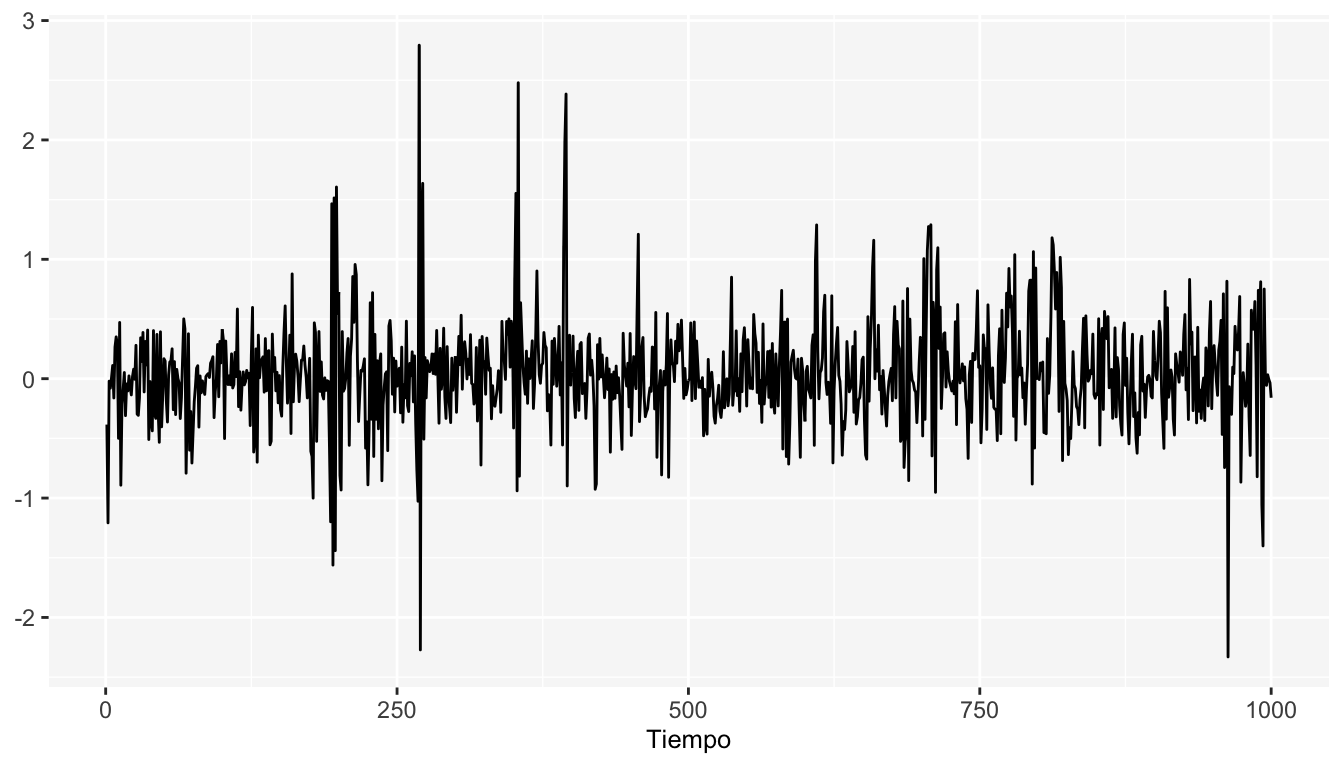
\includegraphics{_main_files/figure-latex/unnamed-chunk-28-1} \end{center}

A continuación se muestran las simulaciones de un modelo \(ARCH(3)\) con la varianza modelada de la siguiente forma: \(\sigma^2_{t}=0.05+ 0.6X_{t-1}+0.2X_{t-2}+0.1X_{t-3}\)

\begin{center}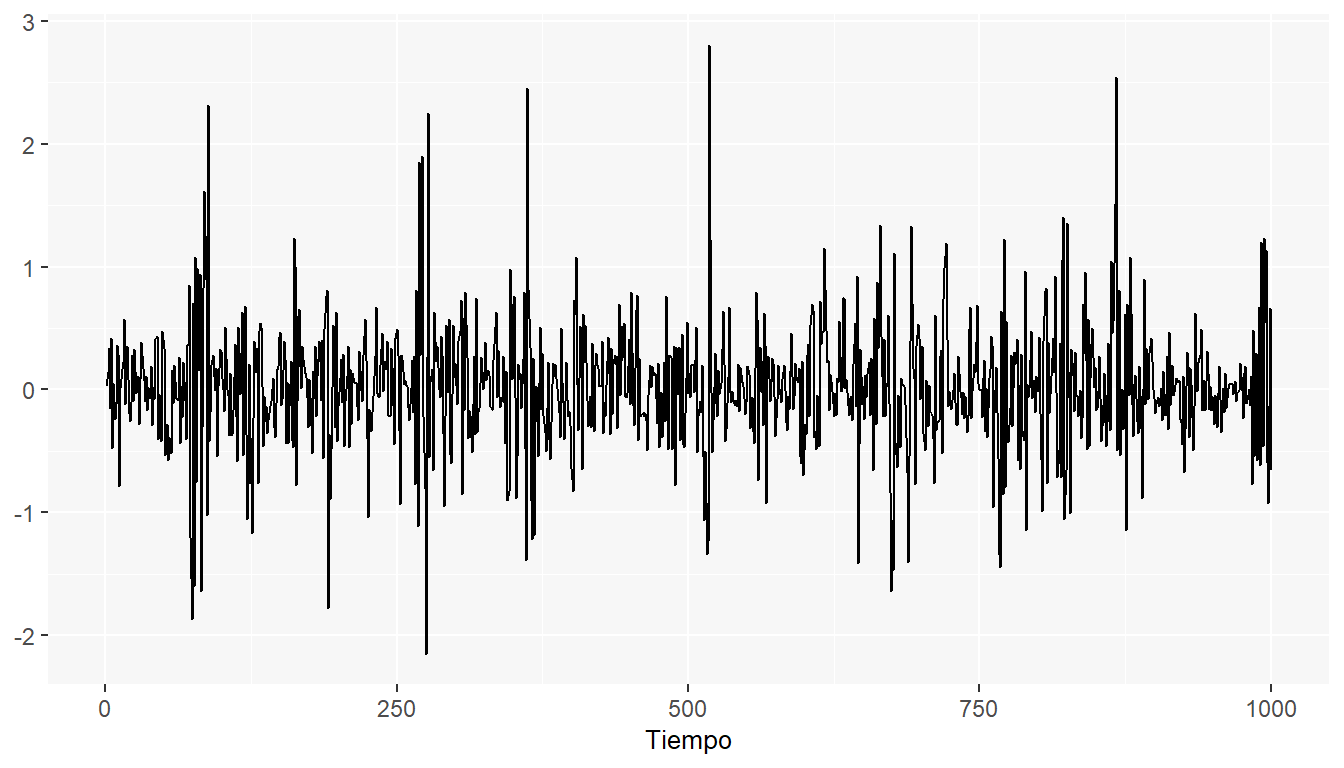
\includegraphics{_main_files/figure-latex/unnamed-chunk-29-1} \end{center}

\hypertarget{garchpq-proceso-autoregresivo-generalizado-con-heterocedasticidad-condicional}{%
\chapter{\texorpdfstring{\(GARCH(p,q)\): Proceso Autoregresivo Generalizado con Heterocedasticidad Condicional}{GARCH(p,q): Proceso Autoregresivo Generalizado con Heterocedasticidad Condicional}}\label{garchpq-proceso-autoregresivo-generalizado-con-heterocedasticidad-condicional}}

En el modelo \(ARCH(1)\) el predictor al tiempo \(t + 1\) de la
varianza depende solo del último valor de \(\sigma_t\). Sin embrago, en la práctica se desea tener mayor precisión en la predicción, para mejorarla se podría incluir todos los valores pasados \(\sigma_t\) con menor peso para volatilidades más distantes.
Una propuesta para este problema la desarrolló Bollerslev(1986), donde introduce \(p\) retrasos de la varianza condicional al modelo, entonces \(p\) hace referencia al orden del modelo GARCH.

Entonces un proceso estacionario \(X_t\) sigue un modelo \(GARCH(p,q)\) si
\[
X_t=\sigma_t\epsilon_t
\]
donde \(\epsilon_t\) es ruido blanco y
\[
\sigma^2_{t} = \alpha_0+\sum_{i=1}^q \alpha_i X^2_{t-i}+\sum_{j=1}^p \beta_j\sigma^2_{t-j}
\]
Donde \(\alpha_0>0\),\(\alpha_i\ge0, i=1,...,q\) y \(\beta_j\ge0, j=1,...,p\). Para garantizar que la varianza sea positiva y existan los momentos de orden superior se requiere que \(\sum_{i=1}^{max(p,q)}(\alpha_i+\beta_i)<1\).

A continuación se muestran las simulaciones de un modelo \(GARCH(1,1)\) con la varianza modelada de la siguiente forma: \(\sigma^2_{t}=0.05+ 0.4X_{t-1}+0.55\sigma^2_{t-1}\)

\begin{center}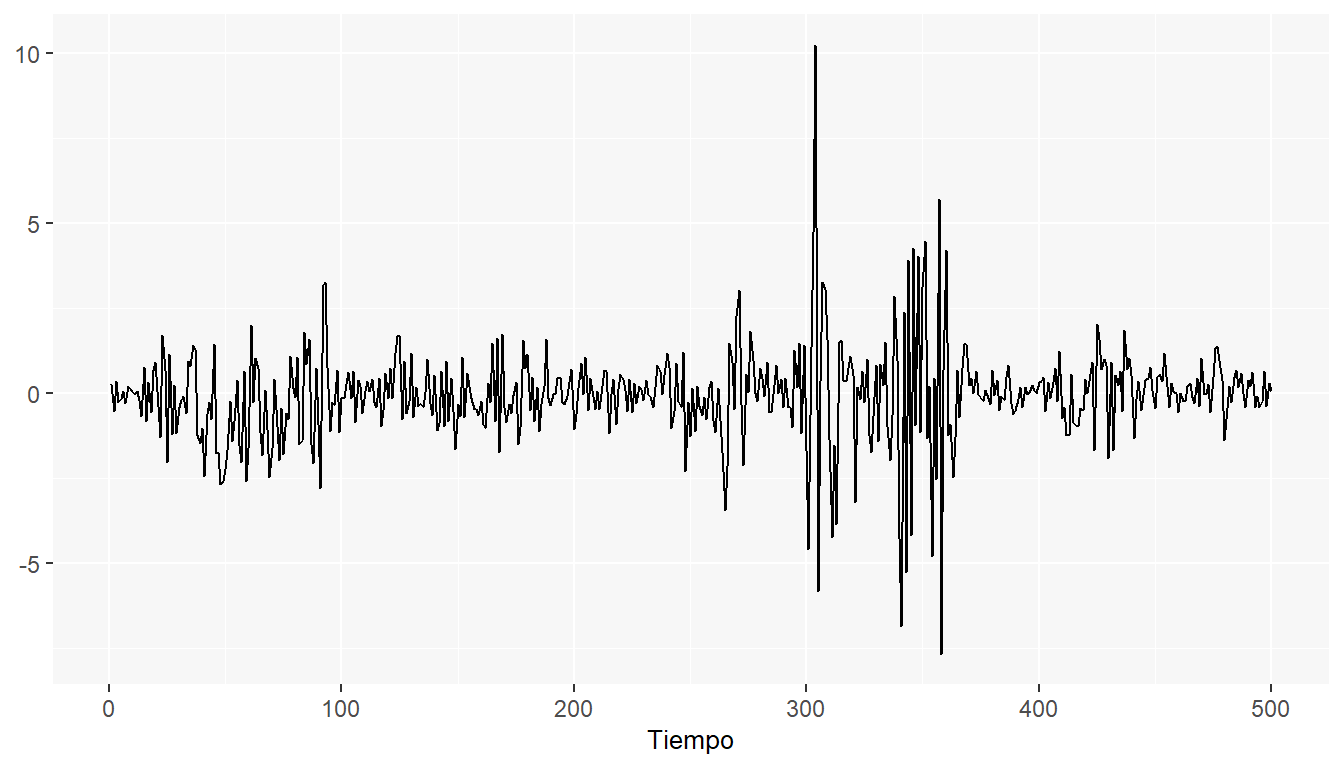
\includegraphics{_main_files/figure-latex/unnamed-chunk-30-1} \end{center}

  \bibliography{book.bib,packages.bib}

\end{document}
